\providecommand{\toplevelprefix}{../..}  %
\documentclass[../../book-main_zh.tex]{subfiles}

\begin{document}

\chapter{优化方法}
\label{app:optimization}

\begin{quote}
    ``{\em 既然整个宇宙的构造是完美的，并且是由智慧的造物主所创造的，那么在宇宙中出现的任何事物，无一不能让人看出某种最大值或最小值的意义。}''

    $~$\hfill -- L. Euler
\end{quote}
\vspace{5mm}

在本章中，我们将简要介绍本书中使用的一些最基础但最重要的优化算法。其目的仅在于帮助读者将这些算法应用于本书所研究的问题，而不是为了深入理解这些算法。因此，我们不会从性能保证的角度对所介绍的算法提供详尽的理论证明。

\section{最速下降法}

优化主要关注如何找到一个函数（例如 \(\cL(\theta)\)）达到其最小值的点。在数学上，这被表述为如下问题：
\begin{equation}
    \argmin_{\theta \in \Theta} \cL(\theta),
\end{equation}
其中 \(\Theta\) 表示自变量 \(\theta\) 所受限制的定义域。通常（除非本章另有说明），\(\Theta\) 简单地取为 \(\R^{n}\)。不失一般性，我们在此假设函数 \(\cL(\theta)\) 是光滑的\footnote{如果函数 \(\cL\) 不是光滑的，我们用所谓的\textit{次梯度}（subgradient）来代替它的梯度。}。

寻找（全局）极小值的效率取决于我们掌握了关于函数 \(\cL\) 的哪些信息。对于本书考虑的大多数优化问题，\(\theta\) 的维度（记为 \(n\)）非常大。这使得计算或获取关于 \(\cL\) 的局部信息变得非常昂贵。特别是，由于梯度 \(\nabla \cL\) 具有 \(n\) 个元素，计算它通常是合理的；然而，海森矩阵（Hessian）\(\nabla^{2} \cL\) 具有 \(n^{2}\) 个元素，计算它通常是极不切实际的（高阶导数也是如此）。因此，通常假设我们拥有零阶信息（即我们能够计算 \(\cL(\theta)\)）和一阶信息（即我们能够计算 \(\nabla \cL(\theta)\)）。优化理论家可能会将其换一种说法，即我们拥有一个“一阶\textit{预言机}（oracle）”。我们在本节介绍的所有优化算法都仅使用一阶预言机。\footnote{关于高维空间中优化算法（包括假设具有高阶预言机的算法）的更系统介绍，我们推荐读者参考 \cite{Wright-Ma-2022} 的著作。}

\subsection{针对光滑问题的朴素梯度下降}

最简单且最广泛使用的优化方法是\textit{梯度下降}（gradient descent, GD）。它最早由柯西（Cauchy）在1847年提出。其思想非常简单：从一个初始状态开始，我们迭代地迈出小步，使得每一步都能减小函数 \(\cL(\theta)\) 的值。

假设当前状态为 \(\theta\)。我们希望在一个由向量 \(\vv\) 指示的方向上迈出一小步（假设距离为 \(h\)），到达一个新状态 \(\theta + h\vv\)，使得函数值减小：
\begin{equation}
    \cL(\theta + h\vv) \leq \cL(\theta).
\end{equation}
为了找到这样的方向 $\vv$，我们可以通过在 \(h = 0\) 处进行泰勒展开来近似 $\cL(\theta +
h\vv)$：
\begin{equation}
    \cL(\theta + h\vv) = \cL(\theta) + h\ip{\nabla \cL(\theta)}{\vv} + o(h),
\end{equation}
其中这里（以及本章中）的内积将是 \(\ell^{2}\) 内积，即 \(\ip{\vx}{\vy} = \vx^{\top}\vy\)。为了找到\textit{最速下降}的方向，我们试图在单位向量 \(\vv\) 中最小化这个泰勒展开式。如果 \(\nabla \cL(\theta) = \vzero\)，那么无论 \(\vv\) 的值是多少，上面的第二项都为 \(0\)，因此我们无法尝试取得进展，即算法已经收敛。另一方面，如果 \(\nabla \cL(\theta) \neq \vzero\)，则有
\begin{equation}\label{eq:steepest_descent_l2_norm}
    \argmin_{\substack{\vv \in \R^{d} \\ \norm{\vv}_{2} = 1}}
    [\cL(\theta) + h\ip{\nabla \cL(\theta)}{\vv}] =
    \argmin_{\substack{\vv \in \R^{d} \\ \norm{\vv}_{2} = 1}}
    \ip{\nabla \cL(\theta)}{\vv} = -\frac{\nabla
    \cL(\theta)}{\norm{\nabla \cL(\theta)}_{2}},
\end{equation}
用文字来说，这意味着对于足够小的 \(h\)，\(\cL(\theta + h\vv)\) 的值沿着方向 \(\vv = -\nabla \cL(\theta)
/ \norm{\nabla \cL(\theta)}_{2}\) 下降得最快。这引出了梯度下降法：从当前状态 \(\theta_{k}\)（\(k=0, 1, \ldots\)）出发，我们在负梯度方向上迈出步长为 \(h\) 的一步，以到达下一个迭代点，
\begin{equation}
    \theta_{k+1} = \theta_{k} - h \nabla \cL(\theta_{k}).
\end{equation}
在机器学习的语境中，步长 \(h\) 也被称为\textit{学习率}（learning rate）。

\subsubsection{步长选择}

剩下的问题是步长 \(h\) 应该是多少？如果我们选择的 \(h\) 太小，函数值可能会下降得非常缓慢，如\Cref{fig:step-size}中间的图所示。如果 \(h\) 太大，函数值甚至可能根本不会下降，如\Cref{fig:step-size}右侧的图所示。

\begin{figure}[ht]
    \centering
    \includegraphics[height=3.5cm]{\toplevelprefix/chapters/appendixA/figs/GD-1.png}
    \hspace{3mm}
    \includegraphics[height=3.5cm]{\toplevelprefix/chapters/appendixA/figs/GD-2.png}
    \hspace{3mm}
    \includegraphics[height=3.5cm]{\toplevelprefix/chapters/appendixA/figs/GD-3.png}
    \caption{（恒定）步长 \(h\) 对梯度下降法收敛性的影响。}
    \label{fig:step-size}
\end{figure}

因此，步长 \(h\) 应该根据函数 \(\cL(\theta_{k})\) 的景观（landscape）来选择。理想情况下，为了选择最佳步长 \(h\)，我们可以求解以下关于单一变量 \(h\) 的优化问题：
\begin{equation}
    h = \argmin_{h^{\prime} \geq 0} \cL(\theta_{k} - h^{\prime}\nabla
    \cL(\theta_{k})).
\end{equation}
这种选择步长的方法被称为\textit{线搜索}（line search）；正如符号所暗示的，它通常用于\textit{在每次迭代 \(k\)} 中获得最优学习率。然而，当函数 \(\cL(\theta_{k})\) 很复杂时（训练深度神经网络时通常如此），在梯度下降的每次迭代中求解这个一维优化问题是非常困难的。

那么我们应该如何选择合适的步长 \(h\) 呢？一种常见且经典的方法是，尝试基于对函数 \(\cL(\theta)\) 整体景观的一些了解，获得当前状态 \(\theta\) 附近局部景观的良好近似。

\begin{figure}
    \centering
    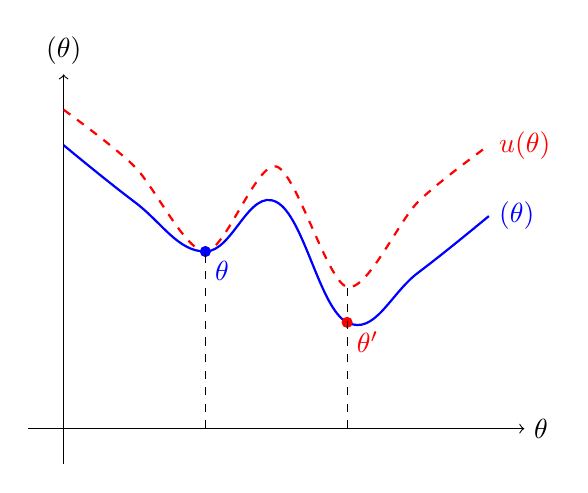
\begin{tikzpicture}[scale=0.9]
        \draw[->] (-0.5,0) -- (6.5,0) node[right] {$\theta$};
        \draw[->] (0,-0.5) -- (0,5) node[above] {$\cL(\theta)$};

        \draw[thick, blue] plot[smooth, tension=0.7] coordinates {
            (0,4) (1,3.2) (2,2.5) (3,3.2) (4,1.5) (5,2.2) (6,3)
        } node[right] {$\cL(\theta)$};

        \draw[thick, red, dashed] plot[smooth, tension=0.5] coordinates {
            (0,4.5) (1,3.7) (2,2.5) (3,3.7) (4,2) (5,3.2) (6,4)
        } node[right] {$u(\theta)$};

        \filldraw[blue] (2,2.5) circle (2pt) node[below right] {$\theta$};

        \filldraw[red] (4,1.5) circle (2pt) node[below right]
        {$\theta^{\prime}$};

        \draw[dashed] (2,0) -- (2,2.5);
        \draw[dashed] (4,0) -- (4,2);
    \end{tikzpicture}
    \caption{\small\textbf{主化-极小化（Majorization-minimization）方案与直观理解。} 函数 \(\cL \colon \Theta \to \R\) 具有一个全局上界 \(u \colon \Theta \to \R\)，该上界至少在一点 \(\theta\) 处与 \(\cL\) 相交。那么，找到使 \(u\) 最小化的 \(\theta^{\prime}\) 将会使 \(\cL\) 的值相比 \(\cL(\theta)\) 得到改善。请注意，关于局部上界也可以证明类似的结果。}
    \label{fig:majorization_minimization}
\end{figure}

关于 \(\cL(\theta)\) 景观的常见条件包括：
\begin{itemize}
    \item \(\alpha\)-强凸性（\(\alpha\)-Strong Convexity）。回想一下，如果 \(\cL\) 的图像位于斜率为 \(\alpha\) 的全局二次下界之上，即对于任意“基点” \(\theta\)，有
        \begin{equation}
            \cL(\theta^{\prime}) \geq l_{\theta,
            \alpha}(\theta^{\prime}) \doteq \cL(\theta) + \ip{\nabla
            \cL(\theta)}{\theta^{\prime} - \theta} +
            \frac{\alpha}{2}\norm{\theta^{\prime} - \theta}_{2}^{2}
        \end{equation}
        我们称 \(\cL\) 是\textit{\(\alpha\)-强凸的}。如果 \(\cL\) 是 \(0\)-强凸的，即其图像位于其切线之上，我们称 \(\cL\) 是\textit{凸的}（convex）。很容易证明（证明留作习题），强凸函数具有唯一的全局极小值。另一个重要的事实（证明留作习题）是，\(\alpha\)-强凸的二阶可导函数 \(\cL\) 具有（对称的）海森矩阵 \(\nabla^{2}\cL\)，其最小特征值 \(\geq \alpha\)。对于 \(\alpha > 0\)，这意味着海森矩阵是对称正定的；对于 \(\alpha = 0\)（即 \(\cL\) 是凸的），这意味着海森矩阵是对称半正定的。
    \item \(\beta\)-利普希茨梯度（\(\beta\)-Lipschitz Gradient，也称为 \(\beta\)-平滑性）。回想一下，如果 \(\nabla \cL\) 存在且是 \(\beta\)-利普希茨连续的，即对于任意“基点” \(\theta\)，有
        \begin{equation}
            \norm{\nabla \cL(\theta^{\prime}) - \nabla
            \cL(\theta)}_{2} \leq \beta \norm{\theta^{\prime} - \theta}_{2}.
        \end{equation}
        我们称 \(\cL\) 具有\textit{\(\beta\)-利普希茨梯度}。很容易证明（证明留作习题），这等价于 \(\cL\) 具有斜率为 \(\beta\) 的全局二次上界，即对于任意“基点” \(\theta\)，有
        \begin{equation}
            \cL(\theta^{\prime}) \leq u_{\theta,
            \beta}(\theta^{\prime}) \doteq \cL(\theta) + \ip{\nabla
            \cL(\theta)}{\theta^{\prime} - \theta} +
            \frac{\beta}{2}\norm{\theta^{\prime} - \theta}_{2}^{2}.
        \end{equation}
        另一个重要的事实（证明留作习题）是，具有 \(\beta\)-利普希茨梯度的凸二阶可导函数具有（对称的）海森矩阵 \(\nabla^{2}\cL\)，其最大特征值 \(\leq \beta\)。
\end{itemize}
首先，让我们假设 \(\cL\) 具有 \(\beta\)-利普希茨梯度（但甚至不一定是凸的）。我们将借此机会介绍一个常见的优化主题：\textit{为了最小化 \(\cL\)，我们可以最小化 \(\cL\) 的一个上界}，这由\Cref{fig:majorization_minimization}中可视化的以下引理所证明。
\begin{lemma}[主化-极小化]\label{lem:majorization_minimization}
    假设 \(u \colon \Theta \to \R\) 是 \(\cL\) 的全局上界，即对于所有 \(\theta \in \Theta\)，有 \(\cL(\theta) \leq u(\theta)\)。假设它们在 \(\theta\) 处相等，即 \(\cL(\theta) = u(\theta)\)。那么
    \begin{equation}
        \theta^{+} \in \argmin_{\theta^{\prime} \in
        \Theta}u(\theta^{\prime}) \implies \cL(\theta^{+}) \leq
        u(\theta^{+}) \leq u(\theta) = \cL(\theta).
    \end{equation}
\end{lemma}

我们将使用这个引理来证明，我们可以利用利普希茨梯度性质来确保每一步梯度更新都不会使 \(\cL\) 的值变差。事实上，在每个基点 \(\theta\) 处，我们有 \(u_{\theta, \beta}\) 是 \(\cL\) 的全局上界，并且 \(u_{\theta, \beta}(\theta) = \cL(\theta)\)。因此，根据\Cref{lem:majorization_minimization}，
\begin{equation}
    \text{if \(\theta^{+}\) minimizes \(u_{\theta, \beta}\) then}
    \quad \cL(\theta^{+}) \leq u_{\theta, \beta}(\theta^{+}) \leq
    u_{\theta, \beta}(\theta) = \cL(\theta).
\end{equation}
这启发了我们，在寻找从 \(\theta_{k}\) 获得 \(\theta_{k + 1}\) 的更新时，我们可以转而最小化关于 \(\theta\) 的上界 \(u_{\theta_{k}, \beta}\)，并将其设为 \(\theta_{k + 1}\)。通过最小化 \(u_{\theta_{k}, \beta}\)（证明留作习题），我们得到
\begin{equation}\label{eq:GD}
    \theta_{k + 1} = \theta_{k} - \frac{1}{\beta}\nabla
    \cL(\theta_{k}) \implies \cL(\theta_{k + 1}) \leq \cL(\theta_{k}).
\end{equation}
这意味着步长 \(h = 1/\beta\) 是一个可用的学习率，但它并没有提供收敛速度，也没有证明 \(\cL(\theta_{k})\) 实际上收敛于 \(\min_{\theta}\cL(\theta)\)。这需要稍微更严格的论证，我们现在就来进行。

现在，让我们假设 \(\cL\) 是 \(\alpha\)-强凸的，具有 \(\beta\)-利普希茨梯度，并且具有全局最优值 \(\theta^{\star}\)。我们将证明 \(\theta_{k}\) 将直接收敛到唯一的全局最优值 \(\theta^{\star}\)，这是一种非常强的收敛形式。特别地，我们将同时使用强凸性和 \(\cL\) 梯度的利普希茨连续性来界定 \(\norm{\theta^{\star} - \theta_{k}}_{2}\)，即观察 \(\theta_{k}\) 周围的邻域：\footnote{在这个证明中，调用 \(\beta\)-利普希茨梯度的步骤略显复杂。我们也将这一步留作习题，提示是将 \(\theta = \theta_{0} - h\nabla \cL(\theta_{0})\) 代入利普希茨梯度恒等式中。}
\begin{align}
    \norm{\theta^{\star} - \theta_{k + 1}}_{2}^{2}
    &\leq \norm{\theta^{\star} - \theta_{k} + h\nabla
    \cL(\theta_{k})}_{2}^{2} \\
    &= \norm{\theta^{\star} - \theta_{k}}_{2}^{2} + 2h\ip{\nabla
    \cL(\theta_{k})}{\theta^{\star} - \theta_{k}} + h^{2}\norm{\nabla
    \cL(\theta_{k})}_{2}^{2} \\
    &\leq \norm{\theta^{\star} - \theta_{k}}_{2}^{2} +
    2h\bp{\cL(\theta^{\star}) - \cL(\theta_{k}) -
    \frac{\alpha}{2}\norm{\theta^{\star} - \theta_{k}}_{2}^{2}} +
    h^{2}\norm{\nabla \cL(\theta_{k})}_{2}^{2} \quad \text{(\(\alpha\)-SC)} \\
    &= \bp{1 - \alpha h}\norm{\theta^{\star} - \theta_{k}}_{2}^{2} +
    2h(\cL(\theta^{\star}) - \cL(\theta_{k})) + h^{2}\norm{\nabla
    \cL(\theta_{k})}_{2}^{2} \\
    &\leq \bp{1 - \alpha h}\norm{\theta^{\star} - \theta_{k}}_{2}^{2}
    + 2h(\cL(\theta^{\star}) - \cL(\theta_{k})) +
    2h^{2}\beta(\cL(\theta_{k}) - \cL(\theta^{\star})) \quad
    \text{(\(\beta\)-LG)} \\
    &= \bp{1 - \alpha h}\norm{\theta^{\star} - \theta_{k}}_{2}^{2} -
    2h(1 - \beta h)(\cL(\theta_{k}) - \cL(\theta^{\star})).
\end{align}
为了确保梯度下降迭代取得进展，我们必须选择步长使得 \(1 - \beta h \geq 0\)，即 \(h \leq 1/\beta\)。如果满足这样的设置，那么
\begin{align}
    \norm{\theta^{\star} - \theta_{k + 1}}_{2}^{2}
    &\leq (1 - \alpha h)\norm{\theta^{\star} - \theta_{k}}_{2}^{2}
    \leq (1 - \alpha h)^{2}\norm{\theta^{\star} - \theta_{k -
    1}}_{2}^{2} \leq \cdots \\
    &\leq (1 - \alpha h)^{k + 1}\norm{\theta^{\star} - \theta_{0}}_{2}^{2}.
\end{align}
为了最小化右侧，我们可以设 \(h = 1/\beta\)，从而得到
\begin{equation}
    \norm{\theta^{\star} - \theta_{k + 1}}_{2}^{2} \leq (1 -
    \alpha/\beta)^{k + 1}\norm{\theta^{\star} - \theta_{0}}_{2}^{2},
\end{equation}
这表明算法以指数衰减的误差收敛到全局最优值。请注意，在这里我们利用收敛速度来获得一个有利的\textit{步长} \(h = 1/\beta\)。这个主题将在本节中反复出现。

我们在本节末尾提出一个警告：学习全局最优值（通常）是不切实际的困难。在某些条件下，我们可以确保梯度下降迭代收敛到一个\textit{局部最优值}。此外，在更宽松的条件下，我们可以确保\textit{局部}收敛，即如果序列初始化得足够接近最优值，迭代将收敛到一个（全局或局部）最优值。

\subsection{针对病态问题的预处理梯度下降}

\begin{figure}
    \includegraphics[width=\textwidth]{\toplevelprefix/chapters/appendixA/figs/hessian_geometry.png}
    \caption{\small\textbf{负梯度 \(-\nabla \cL_{\lambda}\) 与预处理（牛顿法步长）向量场 \(-[\nabla^{2}\cL_{\lambda}]^{-1}[\nabla \cL_{\lambda}]\)}，其中 \(\lambda = 19\)。在空间的某个区域中，沿着负梯度向量场寻找极小值的进展非常微小，但在所有情况下，沿着牛顿法向量场都能以相同的速度向最优值迈进，因为梯度被白化（whitened）了。由于这里的海森矩阵是对角矩阵，自适应学习率算法（例如本节稍后将讨论的 Adam）可以取得与牛顿法相似的进展，但非轴对齐的海森矩阵甚至可能阻碍 Adam 快速成功。}
    \label{fig:hessian_geometry}
\end{figure}

\subsubsection{牛顿法}

对于某些光滑问题和强凸问题，梯度下降的表现仍然相当差。例如，设 \(\lambda \geq 0\)，并设 \(\cL_{\lambda} \colon \R^{2} \to \R\) 的形式为
\begin{equation}
    \cL_{\lambda}(\theta) = \cL_{\lambda}\rp{\mat{\theta_{1}
    \\ \theta_{2}}} \doteq \frac{1}{2}\bc{(1 + \lambda)
    \theta_{1}^{2} + \theta_{2}^{2}} = \frac{1}{2}\theta^{\top}\mat{1
    + \lambda & 0 \\ 0 & 1}\theta.
\end{equation}
这个问题是 \(1\)-强凸的，并且具有 \((1 + \lambda)\)-利普希茨梯度。其收敛速度是几何级数的，速率为 \(1 - 1/(1 + \lambda)\)。对于较大的 \(\lambda\)，这仍然不是很快。在本节中，我们将介绍一类能够成功优化此类病态（badly-conditioned）函数的优化方法。

关键在于目标函数的\textit{曲率}（curvature），它由海森矩阵给出。假设（作为一种反事实情况）我们有一个\textit{二阶}预言机，允许我们计算 \(\cL(\theta)\)、\(\nabla \cL(\theta)\) 和 \(\nabla^{2}\cL(\theta)\)。那么，我们无需选择一个下降方向 \(\vv\) 来优化 \(\theta\) 附近的一阶泰勒展开，而是可以优化二阶泰勒展开。直观地说，这将允许我们将曲率信息纳入更新中。

让我们进行这个计算。\(\cL(\theta + h\vv)\) 在 \(h = 0\) 处的二阶泰勒展开为
\begin{equation}
    \cL(\theta + h\vv) = \cL(\theta) + h\ip{\nabla \cL(\theta)}{\vv}
    + \frac{1}{2}h^{2}\ip{[\nabla^{2}\cL(\theta)]\vv}{\vv} + o(h^{2}).
\end{equation}
然后我们可以计算下降方向：
\begin{align}
    &\argmin_{\substack{\vv \in \R^{n} \\ \norm{\vv}_{2} =
    1}}\bs{\cL(\theta) + h\ip{\nabla \cL(\theta)}{\vv} +
    \frac{1}{2}h^{2}\ip{[\nabla^{2}\cL(\theta)]\vv}{\vv}} \\
    =& \argmin_{\substack{\vv \in \R^{n} \\ \norm{\vv}_{2} =
    1}}\bs{\ip{\nabla \cL(\theta)}{\vv} +
    \frac{1}{2}h\ip{[\nabla^{2}\cL(\theta)]\vv}{\vv}}.
\end{align}
由于约束 \(\norm{\vv}_{2} = 1\)，这个优化问题有点难以求解。但在实践中，我们从不对下降方向 \(\vv\) 进行归一化，而是使用步长 \(h\) 来控制更新的大小。因此，让我们直接在所有向量 \(\vv \in \R^{n}\) 上求解上述问题：\footnote{如果 \(\nabla^{2}\cL(\theta)\) 不可逆，那么我们可以用 \(\nabla^{2}\cL(\theta)\) 的摩尔-彭若斯伪逆（Moore-Penrose pseudoinverse）来代替 \([\nabla^{2}\cL(\theta)]^{-1}\)。}
\begin{equation}
    \argmin_{\vv \in \R^{n}}\bs{\ip{\nabla \cL(\theta)}{\vv} +
    \frac{1}{2}h\ip{[\nabla^{2}\cL(\theta)]\vv}{\vv}} =
    -\frac{1}{h}[\nabla^{2}\cL(\theta)]^{-1}[\nabla \cL(\theta)].
\end{equation}
因此我们可以使用最速下降迭代
\begin{equation}
    \theta_{k + 1} = \theta_{k} -
    [\nabla^{2}\cL(\theta_{k})]^{-1}[\nabla \cL(\theta_{k})],
\end{equation}
（这就是著名的\textit{牛顿法}），或者
\begin{equation}
    \theta_{k + 1} = \theta_{k} -
    h[\nabla^{2}\cL(\theta_{k})]^{-1}[\nabla \cL(\theta_{k})],
\end{equation}
（这被称为\textit{欠阻尼牛顿法}（underdamped Newton's method））。由于二阶二次函数 \(\cL_{\lambda}\) 等于其二阶泰勒展开，如果我们运行牛顿法\textit{一步}，无论 \(\lambda\) 有多大，我们都将在\textit{一步}内达到全局极小值。\Cref{fig:hessian_geometry} 提供了一些关于病态函数以及梯度步长与牛顿步长对比的直观理解。

\subsubsection{预处理梯度下降（PGD）}

在实践中，我们\textit{没有}允许我们计算 \(\nabla^{2}\cL(\theta)\) 的二阶预言机。相反，在从 \(\theta_{k}\) 更新参数到 \(\theta_{k + 1}\) 的同时，我们可以尝试\textit{学习它的一个近似}。

我们如何学习它的近似呢？我们应当找到一些海森矩阵的逆所满足的方程，然后尝试更新我们的近似，使其满足这些方程。也就是说，对 \(\nabla \cL(\theta + \delta_{\theta})\) 在点 \(\theta\) 处进行泰勒展开，我们得到
\begin{equation}
    \underbrace{\nabla \cL(\theta + \delta_{\theta}) - \nabla
    \cL(\theta)}_{\doteq \delta_{\vg}} = [\nabla^{2}
    \cL(\theta)]\delta_{\theta} + o(\norm{\delta_{\theta}}_{2}).
\end{equation}
在这种情况下，我们有
\begin{equation}
    \delta_{\vg} \approx [\nabla^{2}\cL(\theta)]\delta_{\theta}
    \implies \delta_{\theta} \approx [\nabla^{2}\cL(\theta)]^{-1}\delta_{\vg}
\end{equation}
我们现在可以尝试学习一个对称半正定的预处理器（pre-conditioner）\(P \in \R^{n \times n}\)，使得
\begin{equation}
    \delta_{\theta} \approx P\delta_{\vg},
\end{equation}
在每次迭代中与 \(\theta_{k}\) 一起更新它。也就是说，我们有 \textit{PSGD}（预处理随机梯度下降）迭代
\begin{align}
    P_{k}
    &= \mathrm{PreconditionerUpdate}(P_{k - 1}; \theta_{k}, \nabla
    \cL(\theta_{k})) \\
    \theta_{k + 1}
    &= \theta_{k} - hP_{k}\nabla \cL(\theta_{k}).
\end{align}
这种更新存在两个问题：我们如何才能使用 \(P\)（因为我们已经说过无法存储一个 \(n \times n\) 的矩阵），以及我们如何在每次迭代中\textit{更新} \(P\)？答案密切相关；我们永远无法在计算机内存中具体化（materialize）\(P\)，但我们可以使用低秩分解（或类似的方法，如特别适合深度神经网络形式的\textit{克罗内克分解}（Kronecker factorization））来表示它。然后，预处理器更新步骤被设计为利用预处理器表示的结构。

我们在本小节末尾提出一个警告：例如在深度学习中，\(\cL\) 不是一个凸函数，因此牛顿法（及其近似方法）是没有意义的。在这种情况下，我们从凸函数上牛顿法的几何直觉出发，例如从\Cref{fig:hessian_geometry}中可以看出：逆海森矩阵对梯度进行了\textit{白化}。因此，我们可以调整上述过程，学习一种更一般的梯度白化变换，而不是一个近似海森矩阵的预处理器。这就是最初提出 PSGD \cite{li2017preconditioned} 背后的思想（该文献包含了更多关于如何存储和更新预处理器的信息），以及像 Muon \cite{liu2025muon} 这样更现代的优化器的思想。

\subsection{针对非光滑问题的近端梯度下降}\label{subsec:pgd}

然而，即使在非常简单的玩具问题（如 LASSO 或字典学习）中，问题也不是强凸的，而仅仅是凸的，并且目标函数不再仅仅是光滑的，而是一个光滑函数和一个非光滑正则项（如 \(\ell^{1}\) 范数）之和。这类问题可以通过\textit{近端优化算法}（proximal optimization algorithms）来解决，该算法将最速下降法推广到了非光滑目标函数。

形式上，假设
\begin{equation}
    \cL(\theta) \doteq \cS(\theta) + \cR(\theta)
\end{equation}
其中 \(\cS\) 是光滑的，例如具有 \(\beta\)-利普希茨梯度，而 \(\cR\) 是非光滑的（即粗糙的）。近端梯度算法通过使用具有不同全局上界的优化-最小化框架（即\Cref{lem:majorization_minimization}），推广了最速下降算法。也就是说，我们通过提出这样一个问题来构造这样一个上界：如果我们取 \(\cS\) 的利普希茨梯度上界，但\textit{保持 \(\cR\) 不变}会怎样？也就是说，我们有
\begin{equation}
    \cL(\theta^{\prime}) = \cS(\theta^{\prime}) +
    \cR(\theta^{\prime}) \leq u_{\theta, \beta}(\theta^{\prime})
    \doteq \cS(\theta) + \ip{\nabla \cS(\theta)}{\theta^{\prime} -
    \theta} + \frac{\beta}{2}\norm{\theta^{\prime} - \theta}_{2}^{2}
    + \cR(\theta^{\prime}).
\end{equation}
请注意（证明留作习题）
\begin{equation}
    \argmin_{\theta^{\prime}}u_{\theta, \beta}(\theta^{\prime}) =
    \argmin_{\theta^{\prime}}\bs{\frac{\beta}{2}\norm*{\theta^{\prime}
        - \bp{\theta - \frac{1}{\beta}\nabla \cS(\theta)}}_{2}^{2} +
    \cR(\theta^{\prime})}.
\end{equation}
现在，如果我们尝试最小化上界 \(u_{\theta, \beta}\)，我们正在选择一个满足以下条件的 \(\theta^{\prime}\)：
\begin{itemize}
    \item 接近梯度更新 \(\theta - \frac{1}{\beta}\nabla \cS(\theta)\)；
    \item 具有较小的正则项值 \(\cR(\theta^{\prime})\)
\end{itemize}
并根据平滑参数 \(\beta\) 对这些性质进行权衡。因此，让我们定义近端算子（proximal operator）
\begin{equation}
    \prox_{h, \cR}(\theta) \doteq
    \argmin_{\theta^{\prime}}\bs{\frac{1}{2h}\norm{\theta^{\prime} -
    \theta}_{2}^{2} + \cR(\theta^{\prime})}.
\end{equation}
然后，我们可以定义\textit{近端梯度下降}（proximal gradient descent）迭代，在每次迭代中，它最小化上界 \(u_{\theta_{k}, h^{-1}}\)，即
\begin{equation}
    \theta_{k + 1} = \prox_{h, \cR}(\theta_{k} - h\nabla \cS(\theta_{k})).
\end{equation}
当 \(h \leq 1/\beta\) 时，收敛性证明是可能的，但我们在本节中不提供任何证明。

剩下的一个问题是：我们如何计算近端算子？乍一看，我们似乎只是用一个难以处理的最小化问题换取了另一个。由于到目前为止我们没有对 \(\cR\) 做任何假设，即使 \(\cR\) 是一个非常复杂的函数（例如神经网络损失），该框架也能工作，但这将要求我们解决一个神经网络训练问题才能计算单个近端算子。然而，在实践中，对于像我们在本书中使用的简单正则项 \(\cR\)，存在易于计算甚至具有闭式解的近端算子。我们在下面给出几个例子（证明留作习题）。

\begin{example}\label{example:prox-of-characteristic-function}
    设 \(\Gamma \subseteq \Theta\) 为一个集合，并设 \(\chi_{\Gamma}\) 为 \(\Gamma\) 上的特征函数，即
    \begin{equation}
        \chi_{\Gamma}(\theta) \doteq \casework{0, & \text{if}\ \theta
        \in \Gamma \\ +\infty, & \text{if}\ \theta \notin \Gamma.}
    \end{equation}
    那么 \(\chi_{\Gamma}\) 的近端算子是一个投影，即
    \begin{equation}
        \prox_{h, \chi_{\Gamma}}(\theta) = \argmin_{\theta^{\prime}
        \in \Gamma}\frac{1}{2}\norm{\theta^{\prime} - \theta}_{2}^{2}
        = \argmin_{\theta^{\prime} \in \Gamma}\norm{\theta^{\prime} -
        \theta}_{2}.
    \end{equation}
\end{example}

\begin{example}\label{example:prox-of-l1}
    \(\ell^{1}\) 范数具有一个执行软阈值化（soft thresholding）的近端算子：
    \begin{equation}
        S_{h}(\theta) \doteq \prox_{h, \lambda
        \norm{\cdot}_{1}}(\theta) =
        \argmin_{\theta^{\prime}}\bs{\frac{1}{2h}\norm{\theta^{\prime}
        - \theta}_{2}^{2} + \lambda\norm{\theta^{\prime}}_{1}}
    \end{equation}
    那么 \(S_{h}(\theta)\) 按坐标定义为
    \begin{equation}
        S_{h}(\theta)_{i} = \casework{\theta_{i} - h\lambda, &
            \text{if}\ \theta_{i} \geq h\lambda \\ 0, &
            \text{if}\ \theta_{i} \in [-h\lambda, h\lambda] \\ \theta_{i}
        + h\lambda, & \text{if}\ \theta_{i} \leq -h\lambda} =
        \casework{\max\{\abs{\theta_{i}} - h\lambda,
            0\}\sign(\theta_{i}), & \text{if}\ \abs{\theta_{i}} \geq
        h\lambda \\ 0, & \text{if}\ \abs{\theta_{i}} < h\lambda.}
    \end{equation}
    目标函数的光滑部分为最小二乘，非光滑部分为 \(\ell^{1}\) 范数（因此使用这种软阈值近端算子）的近端梯度操作被称为迭代收缩阈值算法（Iterative Shrinkage-Thresholding Algorithm, ISTA）。
\end{example}

\begin{example}\label{example:prox-of-nonnegative-l1}
    在\Cref{ch:deep-networks}中，我们使用了一个对应于 \(\ell^{1}\) 范数加上正卦限（positive orthant）\(\R_{+}^{n} \doteq \{\vx \in
    \R^{n} \colon x_{i} \geq 0\ \forall i\}\) 特征函数的近端算子，即
    \begin{equation}
        T_{h}(\theta) \doteq \prox_{h, \lambda\norm{\cdot}_{1} +
        \chi_{\R_{+}^{n}}}(\theta) = \argmin_{\theta^{\prime} \in
        \R_{+}^{n}}\bs{\frac{1}{2h}\norm{\theta^{\prime} -
        \theta}_{2}^{2} + \lambda\norm{\theta^{\prime}}_{1}},
    \end{equation}
    那么 \(T_{h}\) 定义为
    \begin{equation}
        T_{h}(\theta)_{i} \doteq \max\{\theta_{i} - h\lambda, 0\}.
    \end{equation}
    这个近端算子产生了在\Cref{ch:deep-networks}及后续章节中调用的非负 ISTA。
\end{example}

\subsection{针对大规模问题的随机梯度下降}

在深度学习中，目标函数 \(\cL\) 通常无法精确计算，而是在每个优化步骤中使用有限的样本（例如，使用一个小批量（mini-batch））进行\textit{估计}。对这种情况建模的一种常见方法是定义一个\textit{随机损失函数} \(\cL_{\omega}(\theta)\)，其中 \(\omega\) 是某种“随机性来源”。例如，\(\omega\) 可以包含用于计算损失的批次中样本的索引。然后，我们希望在给定一个\textit{随机一阶预言机}的情况下，关于 \(\theta\) 最小化 \(\cL(\theta) \doteq
\Ex_{\omega}[\cL_{\omega}(\theta)]\)：给定 \(\theta\)，我们可以对 \(\omega\) 进行采样并计算 \(\cL_{\omega}(\theta)\) 和 \(\nabla_{\theta}\cL_{\omega}(\theta)\)。这个最小化问题被称为\textit{随机优化问题}。

基本的一阶随机算法是\textit{随机梯度下降}（stochastic gradient descent, SGD）：在每次迭代 \(k\) 中，我们采样 \(\omega_{k}\)，定义 \(\cL_{k} \doteq \cL_{\omega_{k}}\)，并在 \(\cL_{k}\) 上执行梯度更新，即
\begin{equation}
    \theta_{k + 1} = \theta_{k} - h\nabla \cL_{k}(\theta_{k}).
\end{equation}
然而，即使对于非常简单的问题，我们也无法期望获得与梯度下降相同类型的收敛。例如，假设 \(\omega \in \{1, \dots, m\}\) 有 \(m\) 个可能的值，且取每个值的概率相等，并且有 \(m\) 个可能的目标 \(\xi_{1}, \dots, \xi_{m}\)，使得损失函数 \(\cL_{\omega}\) 为
\begin{equation}
    \cL_{\omega}(\theta) \doteq \frac{1}{2}\norm{\theta - \xi_{\omega}}_{2}^{2}.
\end{equation}
那么 \(\argmin_{\theta}\Ex[\cL_{\omega}(\theta)] = \frac{1}{m}\sum_{i
= 1}^{m}\xi_{i}\)，但随机梯度下降可能会在全局最优值附近“像弹球一样来回震荡（pinball）”，而不会收敛，如\Cref{fig:sgd_nonconvergence}所示。

\begin{figure}
    \includegraphics[width=\textwidth]{\toplevelprefix/chapters/appendixA/figs/sgd_vs_nesterov.png}
    \centering
    \caption{\small\textbf{即使对于非常良好的目标函数，随机梯度下降也可能不收敛，但带动量的 SGD 会收敛。} 即使对于简单的二次目标函数，随机梯度下降的迭代也可能在全局最优值附近来回震荡，而动量平均梯度则会对齐并指向最优值。}
    \label{fig:sgd_nonconvergence}
\end{figure}

为了解决这个问题，我们可以随着时间的推移对参数 \(\theta_{k}\) 进行平均，或者对梯度 \(\nabla
\cL_{k}(\theta_{k})\) 进行平均。如果我们对参数 \(\theta_{k}\) 进行平均，那么（以\Cref{fig:sgd_nonconvergence}作为心智模型）震荡的问题显然是不可能的，因为平均迭代点将越来越靠近中心。因此，大多数理论收敛性证明都考虑平均迭代点 \(\frac{1}{k}\sum_{i = 0}^{k}\theta_{i}\) 向全局极小值的收敛。如果我们对梯度进行平均，我们最终将学习到一个平均梯度 \(\frac{1}{k}\sum_{i = 0}^{k}\nabla
\cL_{k}(\theta_{k})\)，它在每次迭代中变化不大，因此不会发生震荡。

在实践中，我们不使用算术平均，而是对参数采用\textit{指数移动平均}（EMA）（这被称为\textit{波利亚克平均}（Polyak averaging）），或者对梯度采用指数移动平均（这被称为\textit{动量}（momentum））。动量更为流行，我们将在这里对其进行研究。

带动量的随机梯度下降迭代如下：
\begin{align}
    \vg_{k}
    &= \beta\vg_{k - 1} + (1 - \beta)\nabla \cL_{k}(\theta_{k}) \\
    \theta_{k + 1}
    &= \theta_{k} - h\vg_{k}.
\end{align}
我们不进行收敛性证明（示例请参见 \cite{garrigos2023handbook} 的第7章）。然而，动量可以轻松处理我们在\Cref{fig:sgd_nonconvergence}中的玩具案例（见右图）：它停止了震荡，并最终收敛到全局最优值。

我们在末尾提出一个警告：可以证明，对于某些参数设置的选择，Polyak 动量和 Nesterov 动量是等价的。那么也可以证明，在普通 SGD（或 PSGD）中使用衰减的学习率调度（即学习率 \(h\) 依赖于迭代次数 \(k\)，并且当 \(k \to \infty\) 时其极限为 \(h_{k} \to 0\)）可以模拟动量的效果。也就是说，\cite{defazio2023optimal} 证明了如果 SGD 算法持续 \(K\) 次迭代，梯度范数有界 \(\norm{\nabla
\cL(\theta_{k})}_{2} \leq G\)，并且我们定义 \(D \doteq
\norm{\theta_{0} - \theta^{\star}}_{2}\)，那么普通 SGD 的迭代点 \(\theta_{k}\) 满足速率 \(\Ex[\cL(\theta_{k}) -
\cL(\theta^{\star})] \leq DG/\sqrt{K}\) —— 但前提是学习率 \(h_{k} = (D/[G\sqrt{K}])(1 - k/K)\) 随时间\textit{线性}衰减。这与实践中使用的学习率调度相匹配。事实上，令人惊讶的是，这种凸优化理论可以预测深度网络中的许多经验现象 \cite{schaipp2025surprising}，尽管深度学习优化在最坏情况下是高度非凸和非光滑的。目前尚不清楚为什么会这样。

\subsection{将一切结合起来：Adam}

梯度下降方案提出了一种如下形式的迭代
\begin{equation}
    \theta_{k + 1} = \theta_{k} + h\vv_{k},
\end{equation}
其中（回想一下）\(\vv_{k}\) 被选择为（正比于）欧几里得范数下的最速下降向量：
\begin{equation}
    \vv_{k} = -\frac{\nabla \cL(\theta_{k})}{\norm{\nabla
    \cL(\theta_{k})}_{2}} \in \argmin_{\substack{\vv \in \R^{n}
    \\ \norm{\vv}_{2} = 1}}\ip{\nabla \cL(\theta_{k})}{\vv}.
\end{equation}
然而，在深度学习优化的背景下，绝对没有任何理由表明我们必须使用欧几里得范数；事实上，参数空间的“自然几何”并没有被欧几里得范数很好地尊重，因为对于网络的某个特定固定输入，参数空间中的微小变化可能会导致输出空间中的巨大差异。如果我们转而在参数空间 \(\R^{n}\) 上使用一个通用范数 \(\norm{\cdot}\)，我们将得到对应于所谓\textit{对偶范数}（dual norm）的其他量：
\begin{equation}
    \vv_{k} \in \argmin_{\substack{\vv \in \R^{n} \\ \norm{\vv} =
    1}}\ip{\nabla \cL(\theta_{k})}{\vv}.
\end{equation}
例如，如果我们使用 \(\ell^{\infty}\)-范数，可以证明
\begin{equation}
    \vv_{k} = -\sign(\nabla \cL(\theta_{k})) \in
    \argmin_{\substack{\vv \in \R^{n} \\ \norm{\vv}_{\infty} =
    1}}\ip{\nabla \cL(\theta_{k})}{\vv},
\end{equation}
其中 \(\sign(\vx)_{i} = \sign(x_{i}) \in \{-1, 0, 1\}\)。因此，如果我们愿意，我们可以使用所谓的\textit{符号梯度下降}（sign-gradient descent）：
\begin{equation}\label{eq:sign_gradient_descent}
    \theta_{k + 1} = \theta_{k} - h\sign(\nabla \cL(\theta_{k})).
\end{equation}
从符号梯度下降中，我们可以推导出著名的 Adam 优化算法。请注意，对于标量 \(x \in \R\)，我们可以写成
\begin{equation}
    \sign(x) = \frac{x}{\abs{x}} = \frac{x}{\sqrt{x^{2}}}.
\end{equation}
类似地，对于向量 \(\vx \in \R^{n}\)，我们写成（其中 \(\hada\) 和
\(\haddiv\) 分别是逐元素乘法和除法）
\begin{equation}
    \sign(\vx) = \vx \haddiv [\vx^{\hada 2}]^{\hada (1/2)}.
\end{equation}
使用这种表示，我们可以将 \eqref{eq:sign_gradient_descent} 写成
\begin{equation}
    \theta_{k + 1} = \theta_{k} - h ([\nabla \cL(\theta_{k})] \haddiv [\nabla
    \cL(\theta_{k})^{\hada 2}]^{\hada \frac{1}{2}}).
\end{equation}
现在考虑随机情况，即我们在每次迭代中优化不同的损失 \(\cL_{k}\)。在 SGD 中，我们使用动量“跟踪”（即取平均）梯度。在这里，我们可以使用动量同时跟踪梯度和平方梯度，即
\begin{align}
    \vg_{k}
    &= \beta^{1}\vg_{k - 1} + (1 - \beta^{1})\nabla \cL_{k}(\theta_{k}) \\
    \vs_{k}
    &= \beta^{2}\vs_{k - 1} + (1 - \beta^{2})[\nabla
    \cL_{k}(\theta_{k})]^{\hada 2}  \\
    \theta_{k + 1}
    &= \theta_{k} - h\vg_{k}\haddiv\vs_{k}^{\hada \frac{1}{2}},
\end{align}
其中 \(\beta^{i} \in [0, 1]\) 是动量参数。由该迭代给出的算法就是著名的 \textit{Adam} 优化器，\footnote{为了避免除以零的错误，我们除以 \(\vs_{k}^{\hada (1/2)} + \eps \vone_{n}\)，其中 \(\eps\) 是一个很小的值，例如在 \(10^{-8}\) 的数量级。}它是深度学习中最常用的优化器。虽然 Adam 的收敛性证明更为复杂，但它源于我们迄今为止使用的相同最速下降原理，因此我们应该期望，在给定足够小的学习率的情况下，每次更新都应该改善损失。

看待 Adam 的另一种方式（这部分解释了其经验上的成功）是，它根据平方梯度动态更新每个参数的学习率。特别地，请注意我们可以写成
\begin{equation}
    \theta_{k + 1} = \theta_{k} - \eta_{k} \hada \vg_{k} \qquad \text{where}
    \qquad \eta_{k} = h \vs_{k}^{\hada (-\frac{1}{2})}
\end{equation}
其中 \(\eta_{k}\) 是逐参数自适应设置的学习率。这种方案被称为自适应的，因为如果某个特定参数的梯度直到迭代 \(k\) 都很大，那么该参数的学习率就会变小以进行补偿，反之亦然，正如从上式中可以看出。

\section{通过自动微分计算梯度}\label{sec:autodiff}

在上面，我们讨论了几种用于深度网络的优化算法，这些算法假设可以访问\textit{一阶预言机}，即允许我们计算 \(\cL(\theta)\) 和 \(\nabla
\cL(\theta)\) 的机制。对于简单的函数 \(\cL\)，可以手动完成此操作。然而，对于深度神经网络，这很快就会变得繁琐，并阻碍快速实验。因此，我们需要一种通用算法，允许我们高效地计算任意（次）可导网络架构的梯度。

在本节中，我们将介绍\textit{自动微分}（automatic differentiation，AD 或 \textit{autodiff}）的基础知识，这是一种计算一般函数 \(f: \R^{m} \to \R^{n}\) 的梯度和雅可比矩阵（Jacobians）的计算高效方法。我们将展示这如何引出用于计算涉及神经网络的损失函数梯度的反向传播算法。本节结构的摘要如下：
\begin{enumerate}
    \item 我们介绍\textbf{微分}（differentials），这是一种方便的形式化方法，用于计算和组织高维参数空间（它们本身可能是涉及矩阵、张量等其他空间的乘积）之间函数的导数。
    \item 我们描述\textbf{前向模式}（forward-mode）和\textbf{反向模式}（reverse-mode）自动微分的基础知识，其中涉及对于高效计算机器学习应用中出现的不同类型函数的梯度/雅可比矩阵至关重要的考量。
    \item 我们描述在将损失函数应用于层叠式神经网络的特殊情况下的\textbf{反向传播}（backpropagation），作为反向模式自动微分的一个实例。
\end{enumerate}

我们的处理将偏向数学方面，以使读者对底层的数学有深入的理解。读者应确保将这种理解与对深度学习自动微分实践方面的牢固掌握结合起来，例如 \textcite{karpathy-micrograd} 的出色教程中所展示的那样。

\subsection{微分}

本小节的完整说明在优秀的指南 \cite{bright2025matrix} 中给出。为了引入微分，让我们首先考虑一个作用于参数 \(\theta\) 的可导函数 \(\cL \colon
\R \to \R\) 的简单例子。我们可以写成
\begin{equation}
    \cL(\theta^{+}) - \cL(\theta) =
    \cL^{\prime}(\theta)\cdot(\theta^{+} - \theta) +
    o(\abs{\theta^{+} - \theta}).
\end{equation}
如果我们令 \(\delta\theta \doteq \theta^{+} - \theta\) 且 \(\delta\cL \doteq \cL(\theta + \delta\theta) - \cL(\theta)\)，我们可以写成
\begin{equation}
    \delta\cL = \cL^{\prime}(\theta)\cdot\delta\theta + o(\abs{\delta\theta}).
\end{equation}
我们将（非严格地）定义 \(\odif{\theta}\) 和 \(\odif{\cL}\)，即 \(\theta\) 和 \(\cL\) 的\textit{微分}，为 \(\theta\) 和 \(\cL\) 中\textit{无穷小}的变化。可以把它们看作是当 \(\delta\theta\)（以及因此 \(\delta \cL\)）极小时得到的结果。在某种意义上，微分学的目标是研究微分 \(\odif{\theta}\) 和 \(\odif{\cL}\) 之间的关系，即观察函数输入的微小变化如何改变输出。我们应该注意，微分 \(\odif{\theta}\) 与 \(\theta\) 的\textit{形状相同}，微分 \(\odif{\cL}\) 与 \(\cL\) 的\textit{形状相同}。特别地，我们可以写成
\begin{equation}
    \odif{\cL} = \cL^{\prime}(\theta)\cdot\odif{\theta},
\end{equation}
由此我们得出，\(\abs{\odif{\theta}}\) 的所有高次幂，例如 \((\odif{\theta})^{2}\)，都为 \(0\)。

让我们看看这在更高维度（即 \(\cL \colon \R^{n} \to \R\)）下是如何工作的。那么我们仍然有
\begin{equation}
    \odif{\cL} = \cL^{\prime}(\theta)\cdot\odif{\theta}
\end{equation}
对于某种导数概念 \(\cL^{\prime}(\theta)\)。由于这里的 \(\theta\)（因此 \(\odif{\theta}\)）是一个列向量，而 \(\cL\)（因此 \(\odif{\cL}\)）是一个标量，我们必须有 \(\cL^{\prime}(\theta)\) 是一个行向量。在这种情况下，\(\cL^{\prime}(\theta)\) 是 \(\cL\) 关于 \(\theta\) 的雅可比矩阵。这里请注意，我们已将 \(\odif{\theta}\) 坐标的所有高次幂和乘积设为 \(0\)。总之，
\begin{quote}
    \centering
    \textit{微分的所有乘积和 \(\geq 2\) 的幂都等于 \(0\)。}
\end{quote}

现在考虑一个高阶张量函数 \(\cL \colon \R^{m \times n} \to \R^{p \times q}\)。那么我们的基本线性化方程在这种情况下是不够的：\(\odif{\cL} = \cL^{\prime}(\theta) \cdot
\odif{\theta}\) 没有意义，因为 \(\theta\) 是一个 \(m \times n\) 矩阵，而 \(\odif{\cL}\) 是一个 \(p \times q\) 矩阵，因此通常不存在适用于 \(\cL^{\prime}(\theta)\) 的可能向量或矩阵形状（因为没有矩阵可以乘以一个 \(m \times n\) 矩阵来形成一个 \(p \times q\) 矩阵，除非 \(m = p\)）。因此，我们必须有一个稍微更高级的解释。

也就是说，我们将 \(\cL^{\prime}(\theta)\) 视为一个\textit{线性变换}，其输入是 \(\theta\)-空间，输出是 \(\cL\)-空间，它接收 \(\theta\) 的微小变化并输出 \(\cL\) 中相应的微小变化。也就是说，我们可以写成
\begin{equation}
    \odif{\cL} = \cL^{\prime}(\theta)[\odif{\theta}].
\end{equation}
在前面的情况中，\(\cL^{\prime}(\theta)\) 首先是一个线性算子 \(\R \to \R\)，其作用是将其输入乘以 \(\cL\) 关于 \(\theta\) 的标量导数；然后是一个线性算子 \(\R^{n} \to \R\)，其作用是将其输入乘以 \(\cL\) 关于 \(\theta\) 的雅可比导数。一般而言，\(\cL^{\prime}(\theta)\) 是 \(\cL\) 关于 \(\theta\) 的“导数”。可以将 \(\cL^{\prime}\) 视为 \(\cL\) 雅可比矩阵的广义版本。因此，它遵循一些简单的求导法则，最关键的是链式法则。

\begin{theorem}[微分链式法则]
    假设 \(\cL = f \circ g\)，其中 \(f\) 和 \(g\) 是可导的。那么
    \begin{equation}
        \odif{\cL} = f^{\prime}(g(\theta))g^{\prime}(\theta)[\odif{\theta}],
    \end{equation}
    其中（像往常一样）乘法表示线性算子的复合。特别地，
    \begin{equation}
        \cL^{\prime}(\theta) = f^{\prime}(g(\theta))g^{\prime}(\theta)
    \end{equation}
    在线性算子相等的意义上成立。
\end{theorem}

用函子（functorial）的术语来思考多元链式法则是很有成效的：函数的复合被“转化”为雅可比矩阵的矩阵乘法（线性算子的复合！）。我们将通过几个例子来说明这一结果和这种视角的强大之处。

\begin{example}
    考虑函数 \(f(\vX) = \vW\vX + \vb\vone^{\top}\)。那么
    \begin{equation}
        \odif{f} = f(\vX + \odif{\vX}) - f(\vX) = [\vW(\vX +
        \odif{\vX}) + \vb\vone^{\top}] - [\vW \vX + \vb \vone^{\top}]
        = \vW\odif{\vX}.
    \end{equation}
    因此，仿射函数关于其输入的导数为
    \begin{equation}
        f^{\prime}(\vX)[\odif{\vX}] = \vW\odif{\vX} \implies
        f^{\prime}(\vX) = \vW.
    \end{equation}
    请注意，\(f^{\prime}\) 是\textit{常数}。另一方面，考虑函数 \(g(\vW, \vb) = \vW\vX + \vb\vone^{\top}\)。那么
    \begin{align}
        \odif{g}
        &= g(\vW + \odif{\vW}, \vb + \odif{\vb}) - g(\vW, \vb) 
        \\
        &=
        [(\vW + \odif{\vW})\vX + (\vb + \odif{\vb})\vone^{\top}] -
        [\vW\vX + \vb\vone^{\top}] \\
        &= (\odif{\vW})\vX + (\odif{\vb})\vone^{\top} =
        g^{\prime}(\vW, \vb)[\odif{\vW}, \odif{\vb}].
    \end{align}
    请注意，这个导数关于 \(\vW, \vb\) 是\textit{常数}（这是合理的，因为 \(g\) 本身是线性的），并且关于微分输入 \(\odif{\vW}, \odif{\vb}\) 是线性的。
\end{example}

\begin{example}
    考虑函数 \(f = gh\)，其中 \(g, h\) 是输出可以相乘的可导函数。那么 \(f = p \circ v\)，其中 \(v = (g, h)\) 且 \(p(a, b) = ab\)。应用链式法则，我们有
    \begin{equation}
        \odif{f} = p^{\prime}(v(x))v^{\prime}(x)[\odif{x}].
    \end{equation}
    为了计算 \(v^{\prime}(x)\)，我们可以计算
    \begin{equation}
        \odif{v} = v^{\prime}(x)[\odif{x}] = v(x + \odif{x}) - v(x) =
        \mat{g(x + \odif{x}) - g(x) \\ h(x + \odif{x}) - h(x)} =
        \mat{g^{\prime}(x)[\odif{x}] \\ h^{\prime}(x)[\odif{x}]}.
    \end{equation}
    为了计算 \(p^{\prime}\)，我们可以计算
    \begin{align}
        \odif{p}
        &= p^{\prime}(a, b)[\odif{a}, \odif{b}] = p(a + \odif{a}, b +
        \odif{b}) - p(a, b) = (a + \odif{a})(b + \odif{b}) - ab \\
        &= (\odif{a})b + a(\odif{b}) + (\odif{a})(\odif{b}) =
        (\odif{a})b + a(\odif{b}),
    \end{align}
    其中（回想一下）微分 \(\odif{a}\) 和 \(\odif{b}\) 的乘积被设为 \(0\)。因此
    \begin{equation}
        p^{\prime}(a, b)[\odif{a}, \odif{b}] = (\odif{a})b + (\odif{b})a.
    \end{equation}
    将这些结合起来，我们发现
    \begin{align}
        f^{\prime}(x)[\odif{x}]
        &= p^{\prime}(v(x))v^{\prime}(x)[\odif{x}] = p^{\prime}(g(x),
        h(x))[g^{\prime}(x)[\odif{x}], h^{\prime}(x)[\odif{x}]] \\
        &= (g^{\prime}(x)[\odif{x}])h(x) + g(x)(h^{\prime}(x)[\odif{x}]).
    \end{align}
    这给出了
    \begin{equation}
        f^{\prime}(x)[\odif{x}] = (g^{\prime}(x)[\odif{x}])h(x) +
        g(x)(h^{\prime}(x)[\odif{x}]).
    \end{equation}
    例如，如果我们说 \(f, g, h \colon \R \to \R\)，那么所有项都是可交换的，因此
    \begin{equation}
        f^{\prime}(x)[\odif{x}] = (g^{\prime}(x)h(x) +
        g(x)h^{\prime}(x))[\odif{x}] \implies f^{\prime}(x) =
        g^{\prime}(x)h(x) + g(x)h^{\prime}(x)
    \end{equation}
    这就是我们熟悉的乘积法则。
\end{example}

\begin{example}
    考虑函数 \(f(\vA) = \vA^{\top}\vA\vB\vA\)，其中
    \(\vA\) 是一个矩阵，\(\vB\) 是一个常数矩阵。那么，
    令 \(f = gh\)，其中 \(g(\vA) = \vA^{\top}\vA\) 且 \(h(\vA)
    = \vB\vA\)，我们可以使用乘积法则得到
    \begin{align}
        f^{\prime}(\vA)[\odif{\vA}]
        &= (g^{\prime}(\vA)[\odif{\vA}])h(\vA) +
        g(\vA)(h^{\prime}(\vA)[\odif{\vA}]) \\
        &= ((\odif{\vA})^{\top}\vA + \vA^{\top}(\odif{\vA}))\vB\vA +
        \vA^{\top}\vA\vB(\odif{\vA}).
    \end{align}
\end{example}

\begin{example}
    考虑由下式给出的函数 \(f \colon \R^{m \times n \times k} \to
    \R^{m \times n}\)
    \begin{equation}
        f(\vA)_{ij} = \sum_{t = 1}^{k}A_{ijt}.
    \end{equation}
    我们无法为该函数写出（矩阵值的）雅可比矩阵或梯度。但我们可以很好地计算它的微分：
    \begin{equation}
        \odif{f}_{ij} = [f(\vA + \odif{\vA}) - f(\vA)]_{ij} = \sum_{t
        = 1}^{k}\odif{\vA}_{ijt} = \vone_{k}^{\top}(\odif{\vA})_{ij}.
    \end{equation}
    因此
    \begin{equation}
        (f^{\prime}(\vA)[\odif{\vA}])_{ij} = \vone_{k}^{\top}(\odif{\vA})_{ij},
    \end{equation}
    这表示一个高阶张量乘法操作，尽管如此，它仍然是良定义的。
\end{example}

这为我们提供了计算所有事物微分所需的所有技术。
本节我们要讨论的最后一件事是使用微分计算梯度的方法。即，对于输出为标量的函数 \(\cL\)，其梯度 \(\nabla \cL\) 定义为
\begin{equation}
    \odif{\cL} = \cL^{\prime}(\theta)[\odif{\theta}] = \ip{\nabla
    \cL(\theta)}{\odif{\theta}},
\end{equation}
这里的内积是指定对象的“标准”内积（即，对于向量，它是 \(\ell^{2}\) 内积；对于矩阵，它是 Frobenius 内积；对于高阶张量，它是类似的坐标和内积）。
这个定义是我们将从 $\R^n$ 到 $\R$ 的函数的梯度视为偏导数向量这一“熟悉”例子的正确推广——针对一般函数 $f : \R^m \to
\R^n$ 的泰勒定理的一个版本使这种联系变得严密。
因此，计算梯度 \(\nabla \cL\) 的一种方法是计算微分 \(\odif{\cL}\) 并将其重写为 \(\ip{\text{something}}{\odif{\theta}}\) 的形式，那么那个“something”就是梯度。

\subsection{自动微分}

自动微分（AD）的主要思想是高效地计算链式法则。
我们需要处理的基本问题如下。在附录的优化部分中，我们认为参数空间 \(\Theta\) 是一个抽象的欧几里得空间，如 \(\R^{n}\)。在实践中，参数实际上是向量、矩阵和高阶对象的某种集合：\(\Theta = \R^{m \times n} \times \R^{n}
\times \R^{r \times q \times p} \times \R^{r \times q} \times \cdots\)。虽然在理论上，这与某个（非常大的）\(n^{\prime}\) 对应的大参数空间 \(\R^{n^{\prime}}\) 是同一回事，但计算上高效的微分算法必须对这两个空间区别对待。
前向模式和反向模式自动微分是执行此计算的两种不同方案。

让我们从一个简单的例子开始。令 \(\cL\) 定义为 \(\cL
= a \circ b \circ c\)，其中 \(a, b, c\) 是可微的。那么\textit{链式法则}给出
\begin{equation}
    \cL^{\prime}(\theta) =
    a^{\prime}(b(c(\theta)))b^{\prime}(c(\theta))c^{\prime}(\theta).
\end{equation}
为了计算 \(\cL(\theta)\)，我们首先计算 \(c(\theta)\)，然后计算 \(b(c(\theta))\)，接着计算 \(a(b(c(\theta)))\)，并将它们全部存储起来。计算 \(\cL^{\prime}(\theta)\) 有两种方法。\textit{前向模式自动微分}将计算
\begin{equation}
    c^{\prime}(\theta) \implies
    b^{\prime}(c(\theta))c^{\prime}(\theta) \implies
    a^{\prime}(b(c(\theta)))b^{\prime}(c(\theta))c^{\prime}(\theta)
\end{equation}
即“自底向上”地计算导数。\textit{反向模式自动微分}将计算
\begin{equation}
    a^{\prime}(b(c(\theta))) \implies
    a^{\prime}(b(c(\theta)))b^{\prime}(c(\theta)) \implies
    a^{\prime}(b(c(\theta)))b^{\prime}(c(\theta))c^{\prime}(\theta),
\end{equation}
即“自顶向下”地计算导数。为了理解为什么这很重要，假设 \(f \colon \R^{p} \to \R^{s}\) 由 \(f = a \circ b \circ c\) 给出，其中 \(a \colon \R^{r} \to \R^{s}\)，\(b
\colon \R^{q} \to \R^{r}\)，\(c \colon \R^{p} \to \R^{q}\)。那么链式法则为：
\begin{equation}
    f^{\prime}(\vx) = a^{\prime}(b(c(\vx)))b^{\prime}(c(\vx))c^{\prime}(\vx)
\end{equation}
其中（回想一下）\(f^{\prime}\) 是导数，在这种情况下是雅可比矩阵（因为每个函数的输入和输出都是向量）。假设计算每个雅可比矩阵是微不足道的，唯一的代价是将雅可比矩阵相乘，前向模式自动微分具有以下计算成本（假设将 \(A \in
\R^{m \times n}, B \in \R^{n \times k}\) 相乘需要 \(\cO(mnk)\) 时间）：
\begin{align}
    &\text{computing}\ c^{\prime}(\vx) \in \R^{q \times
    p}\ \text{takes negligible time} \\
    &\text{computing}\ b^{\prime}(c(\vx))c^{\prime}(x) \in \R^{r
    \times p}\ \text{takes \(\cO(pqr)\) time} \\
    &\text{computing}\ a^{\prime}(b(c(\vx)))b^{\prime}(c(\vx))c^{\prime}(\vx)
    \in \R^{s \times p}\ \text{takes \(\cO(pqr + prs)\) time.}
\end{align}
同时，执行反向模式自动微分具有以下计算成本：
\begin{align}
    &\text{computing}\ a^{\prime}(b(c(\vx))) \in \R^{s \times
    r}\ \text{takes negligible time} \\
    &\text{computing}\ a^{\prime}(b(c(\vx)))b^{\prime}(c(\vx)) \in
    \R^{s \times q}\ \text{takes \(\cO(qrs)\) time} \\
    &\text{computing}\ a^{\prime}(b(c(\vx)))b^{\prime}(c(\vx))c^{\prime}(\vx)
    \in \R^{s \times p}\ \text{takes \(\cO(qrs + pqs)\) time.}
\end{align}
换句话说，前向模式自动微分需要 \(\cO(p(qr + rs))\) 时间，而反向模式自动微分需要 \(\cO(s(pq + qr))\) 时间。\textit{它们花费的时间是不同的！}

更一般地，假设 \(f = f^{L} \circ \cdots \circ f^{1}\)，其中每个 \(f^{\ell} \colon \R^{d^{\ell - 1}} \to \R^{d^{\ell}}\)，因此 \(f \colon \R^{d^{0}} \to \R^{d^{L}}\)。那么前向模式自动微分需要 \(\cO(d^{0}(\sum_{\ell = 2}^{L}d^{\ell - 1}d^{\ell}))\) 时间，而反向模式自动微分需要 \(\cO(d^{L}(\sum_{\ell = 1}^{L -
1}d^{\ell - 1}d^{\ell}))\) 时间。从上述速率可以看出，在其他条件相同的情况下：
\begin{itemize}
    \item 如果要优化的函数\textit{输出多于输入}（即 \(d^{L} > d^{0}\)），请使用\textit{前向模式自动微分}。
    \item 如果要优化的函数\textit{输入多于输出}（即 \(d^{0} > d^{L}\)），请使用\textit{反向模式自动微分}。
\end{itemize}
在神经网络中，我们计算\textit{损失函数} \(\cL \colon \Theta \to \R\) 的梯度，其中参数空间 \(\Theta\) 通常是非常高维的。因此在实践中，我们总是使用反向模式自动微分来训练神经网络。在训练神经网络的语境下，反向模式自动微分被称为\textit{反向传播}。

\subsection{反向传播}
\label{app:BP-section}
在本节中，我们将使用一个简单但完全实用的例子来讨论算法化的反向传播。假设我们固定一个输入-标签对 \((\vX, \vy)\)，并固定一个网络架构 \(f_{\theta} = f_{\theta}^{L} \circ \cdots \circ f_{\theta}^{1} \circ
f_{\theta}^{\emb}\)，其中 \(\theta = (\theta^{\emb}, \theta^{1},
\dots, \theta^{L}, \theta^{\head})\) 且特定任务头为 \(h_{\theta^{\head}}\)，并记
\begin{align}
    &\vZ_{\theta}^{1}(\vX) \doteq f_{\theta}^{\emb}(\vX), \\
    &\vZ_{\theta}^{\ell + 1}(\vX) \doteq
    f_{\theta}^{\ell}(\vZ_{\theta}^{\ell}(\vX)), \quad \forall \ell
    \in \{1, \dots, L\}, \\
    &\hat{\vy}_{\theta^{\head}}(\vX) \doteq h_{\theta^{\head}}(\vZ_{\theta}^{L+1}(\vX)).
\end{align}
那么，我们可以将这一项的损失定义为
\begin{equation}
    \cL(\theta) \doteq \sfL(\vy, \hat{\vy}_{\theta}(\vX)),
\end{equation}
其中 \(\sfL\) 是关于其第二个参数的可微函数。那么反向模式自动微分指示我们按照 \(\theta^{\head}, \theta^{L}, \dots, \theta^{1}, \theta^{\emb}\) 的顺序计算导数。

为了执行此计算，让我们对符号进行一些更改。
\begin{itemize}
    \item 首先，让我们更改符号以强调变量之间的依赖结构。即，
        \begin{align}
            &\vZ^{1} \doteq f^{\emb}(\vX, \theta^{\emb}) \\
            &\vZ^{\ell + 1} \doteq f^{\ell}(\vZ^{\ell},
            \theta^{\ell}), \qquad \forall \ell \in \{1, \dots, L\}, \\
            &\hat{\vy} \doteq h(\vZ^{L+1}, \theta^{\head}), \\
            &\cL \doteq \sfL(\vy, \hat{\vy}).
        \end{align}
    \item 其次，我们不再将导数记为 \(f^{\prime}\)，而是显式地标出自变量，例如将导数写为 \(\odv{f}{\theta^{1}}\)。这是因为我们的模型中有很多变量，而我们每次只关心一个。
\end{itemize}
我们可以从计算适当的微分开始。首先，对于 \(\theta^{\head}\)，我们有
\begin{align}
    \odif{\cL}
    &= \odif{\sfL} \\
    &= \odv{\sfL}{\hat{\vy}}\cdot\odif{\hat{\vy}} \\
    &= \odv{\sfL}{\hat{\vy}}\cdot\odif{{(h(\vZ^{L + 1}, \theta^{\head}))}} \\
    &= \odv{\sfL}{\hat{\vy}}\bs{\odv{h}{\vZ^{L +
        1}}\cdot\odif{\vZ}^{L + 1} +
    \odv{h}{\theta^{\head}}\cdot\odif{\theta}^{\head}}.
\end{align}
现在，由于 \(\vZ^{L + 1}\) 不依赖于 \(\theta^{\head}\)，我们有 \(\odif{\vZ}^{L + 1} = 0\)，因此最终成立（利用对于陪域为 \(\R\) 的函数 \(\sfL\)，梯度是导数的转置这一事实）：
\begin{align}
    \odif{\cL}
    &=
    \odv{\sfL}{\hat{\vy}}\cdot\odv{h}{\theta^{\head}}\cdot\odif{\theta}^{\head}
    \\
    &=
    [\nabla_{\hat{\vy}}\sfL]^{\top}\odv{h}{\theta^{\head}}\cdot\odif{\theta}^{\head}
    \\
    &=
    \ip*{\nabla_{\hat{\vy}}\sfL}{\odv{h}{\theta^{\head}}\cdot\odif{\theta}^{\head}}
    \\
    &=
    \ip*{\bp{\odv{h}{\theta^{\head}}}^{*}\nabla_{\hat{\vy}}\sfL}{\odif{\theta}^{\head}}
    \\
    &= \ip{\nabla_{\theta^{\head}}\cL}{\odif{\theta}^{\head}}.
\end{align}
因此，为了计算 \(\nabla_{\theta^{\head}}\cL\)，我们计算梯度 \(\nabla_{\hat{\vy}}\sfL\) 以及导数 \(\odv{h}{\theta^{\head}}\) 的\textit{伴随}（adjoint）\footnote{伴随类似于更一般线性变换的广义转置。特别地，对于给定的一对内积空间和这些空间之间的线性变换 \(T\)，伴随 \(T^{*}\) 由恒等式 \(\ip{T\vx}{\vy} = \ip{\vx}{T^{*}\vy}\) 定义。在有限维（即与本书相关的所有情况）中，伴随存在且唯一。}并相乘（即，将伴随线性变换应用于梯度）。在实践中，这两个导数都可以手工计算，但许多现代计算框架可以在给定“前向传播”（即损失函数计算）代码的情况下\textit{自动}定义导数（和/或它们的伴随）。虽然将这种自动导数定义扩展到尽可能多的函数是一个活跃的研究领域，但文献 \cite{bright2025matrix} 详细描述了实现它的一种基本方法。顺便说一下，反向传播也因此被称为\textit{伴随方法}（adjoint method）——即我们使用伴随导数来计算梯度。

现在让我们计算关于某个 \(\theta^{\ell}\) 的微分：
\begin{align}
    \odif{\cL}
    &= \odv{\cL}{\vZ^{\ell + 1}}\cdot \odif{\vZ^{\ell + 1}} \\
    &= \odv{\cL}{\vZ^{\ell + 1}}\cdot \odif{{(f^{\ell}(\vZ^{\ell},
    \theta^{\ell}))}} \\
    &= \odv{\cL}{\vZ^{\ell +
    1}}\bs{\odv{f^{\ell}}{\vZ^{\ell}}\cdot\odif{\vZ}^{\ell} +
    \odv{f^{\ell}}{\theta^{\ell}}\cdot\odif{\theta}^{\ell}} \\
    &= \odv{\cL}{\vZ^{\ell + 1}}\cdot
    \odv{f^{\ell}}{\theta^{\ell}}\cdot\odif{\theta}^{\ell} \qquad
    \text{(b/c~\(\vZ^{\ell}\) isn't fn.~of \(\theta^{\ell}\) so
    \(\odif{\vZ}^{\ell} = 0\))} \\
    &= [\nabla_{\vZ^{\ell +
    1}}\cL]^{\top}\odv{f^{\ell}}{\theta^{\ell}}\cdot\odif{\theta}^{\ell} \\
    &= \ip*{\nabla_{\vZ^{\ell +
    1}}\cL}{\odv{f^{\ell}}{\theta^{\ell}}\cdot\odif{\theta}^{\ell}} \\
    &= \ip*{\bp{\odv{f^{\ell}}{\theta^{\ell}}}^{*}\nabla_{\vZ^{\ell +
    1}}\cL}{\odif{\theta}^{\ell}} \\
    &= \ip{\nabla_{\theta^{\ell}}\cL}{\odif{\theta}^{\ell}}.
\end{align}
因此，为了计算 \(\nabla_{\theta^{\ell}}\cL\)，我们计算 \(\nabla_{\vZ^{\ell + 1}}\cL\)，然后将伴随导数 \(\bp{\odv{f^{\ell}}{\theta^{\ell}}}^{*}\) 应用于它。由于 \(\nabla_{\theta^{\ell}}\cL\) 依赖于 \(\nabla_{\vZ^{\ell +
1}}\cL\)，我们还希望能够计算关于 \(\vZ^{\ell}\) 的梯度。这可以用完全相同的方式计算：
\begin{align}
    \odif{\cL}
    &= \odv{\cL}{\vZ^{\ell + 1}}\cdot \odif{\vZ^{\ell + 1}} \\
    &= \odv{\cL}{\vZ^{\ell + 1}}\cdot\odif{{(f^{\ell}(\vZ^{\ell},
    \theta^{\ell}))}} \\
    &= \odv{\cL}{\vZ^{\ell +
    1}}\bs{\odv{f^{\ell}}{\vZ^{\ell}}\cdot\odif{\vZ}^{\ell} +
    \odv{f^{\ell}}{\theta^{\ell}}\cdot\odif{\theta}^{\ell}} \\
    &= \odv{\cL}{\vZ^{\ell +
    1}}\cdot\odv{f^{\ell}}{\vZ^{\ell}}\cdot\odif{\vZ}^{\ell} \qquad
    \text{(b/c~~\(\theta^{\ell}\) isn't fn.~of \(\vZ^{\ell}\) so
    \(\odif{\theta}^{\ell} = 0\) this time)} \\
    &= \ip*{\bp{\odv{f^{\ell}}{\vZ^{\ell}}}^{*}\nabla_{\vZ^{\ell +
    1}}\cL}{\odif{\vZ}^{\ell}} \qquad \text{(same machine)} \\
    &= \ip{\nabla_{\vZ^{\ell}}\cL}{\odif{\vZ}^{\ell}}.
\end{align}
因此，为了计算 \(\nabla_{\vZ^{\ell}}\cL\)，我们计算 \(\nabla_{\vZ^{\ell + 1}}\cL\)，然后将伴随导数 \(\bp{\odv{f^{\ell}}{\vZ^{\ell}}}^{*}\) 应用于它。所以我们得到了一个计算所有 \(\ell\) 的 \(\nabla_{\vZ^{\ell}}\cL\) 的递归，其基本情况为 \(\nabla_{\vZ^{L + 1}}\cL\)，由下式给出
\begin{align}
    \odif{\cL}
    &= \odif{\sfL} \\
    &= \odv{\sfL}{\hat{\vy}}\cdot\odif{\hat{\vy}} \\
    &= \odv{\sfL}{\hat{\vy}}\cdot\odif{{h(\vZ^{L + 1}, \theta^{\head})}} \\
    &= \odv{\sfL}{\hat{\vy}}\bs{\odv{h}{\vZ^{L +
        1}}\cdot\odif{\vZ}^{L + 1} +
    \odv{h}{\theta^{\head}}\cdot\odif{\theta}^{\head}} \\
    &= \odv{\sfL}{\hat{\vy}}\cdot \odv{h}{\vZ^{L + 1}}\cdot\odif{\vZ}^{L + 1} \\
    &= \ip*{\bp{\odv{h}{\vZ^{L +
    1}}}^{*}\nabla_{\hat{\vy}}\sfL}{\odif{\vZ}^{L + 1}} \\
    &= \ip{\nabla_{\vZ^{L + 1}}\cL}{\odif{\vZ}^{L + 1}}.
\end{align}
因此我们得到递归：
\begin{align}
    \nabla_{\vZ^{L + 1}}\cL
    &= \bp{\odv{h}{\vZ^{L + 1}}}^{*}\nabla_{\hat{\vy}}\sfL \\
    \nabla_{\vZ^{L}}\cL
    &= \bp{\odv{f^{L}}{\vZ^{L}}}^{*}\nabla_{\vZ^{L + 1}}\cL \\
    \nabla_{\theta^{L}}\cL
    &= \bp{\odv{f^{L}}{\theta^{L}}}^{*}\nabla_{\vZ^{L + 1}}\cL \\
    \vdots &  \\
    \nabla_{\vZ^{1}}\cL
    &= \bp{\odv{f^{1}}{\vZ^{1}}}^{*}\nabla_{\vZ^{2}}\cL \\
    \nabla_{\theta^{1}}\cL
    &= \bp{\odv{f^{1}}{\theta^{1}}}^{*}\nabla_{\vZ^{2}}\cL \\
    \nabla_{\theta^{\emb}}\cL
    &= \bp{\odv{f^{\emb}}{\theta^{\emb}}}^{*}\nabla_{\vZ^{1}}\cL.
\end{align}

这为我们提供了一种计算高效的算法，用于寻找整个网络中的所有梯度。

我们将通过计算一个简单层的伴随导数来结束本节。
\begin{example}
    考虑“线性”（仿射）层 \(f^{\ell}\)
    \begin{equation}
        f^{\ell}(\vZ, \vW^{\ell}, \vb^{\ell}) \doteq \vW^{\ell}\vZ +
        \vb^{\ell}\vone^{\top} = \mat{\vW^{\ell} & \vb^{\ell}}.
    \end{equation}
    我们可以计算关于这两个参数的微分如下
    \begin{align}
        \odif{f}^{\ell}
        &= [(\vW^{\ell} + \odif{\vW}^{\ell})\vZ + (\vb^{\ell} +
        \odif{\vb}^{\ell})\vone^{\top}] - [\vW^{\ell}\vZ + \vb^{\ell}\vone^{\top}] \\
        &= (\odif{\vW}^{\ell})\vZ + (\odif{\vb}^{\ell})\vone^{\top}.
    \end{align}
    因此，该变换的导数为
    \begin{equation}
        \odv{f^{\ell}}{(\vW^{\ell}, \vb^{\ell})}[\odif{\vW}^{\ell},
        \odif{\vb}^{\ell}] = (\odif{\vW}^{\ell})\vZ +
        (\odif{\vb}^{\ell})\vone^{\top},
    \end{equation}
    即，表示以下从 \(\R^{m \times d} \times \R^{m}\) 到 \(\R^{m \times n}\) 的线性变换：
    \begin{equation}
        T[\vA, \vu] = \vA\vZ + \vu\vone^{\top}.
    \end{equation}
    我们通过以下过程计算关于坐标和（Frobenius）内积的伴随 \(T^{*} \colon \R^{m \times n} \to \R^{m
    \times d} \times \R^{m}\)：
    \begin{align}
        \ip{T[\vA, \vu]}{\vB}_{\R^{m \times n}}
        &= \tr((\vA\vZ + \vu\vone^{\top})\vB^{\top}) \\
        &= \tr(\vA\vZ\vB^{\top} + \vu\vone^{\top}\vB^{\top}) \\
        &= \tr(\vA\vZ\vB^{\top}) + \tr(\vu\vone^{\top}\vB^{\top}) \\
        &= \tr(\vB\vZ^{\top}\vA^{\top}) + \tr(\vone^{\top}\vB^{\top}\vu) \\
        &= \ip{\vB\vZ^{\top}}{\vA}_{\R^{m \times d}} +
        \ip{\vB\vone}{\vu}_{\R^{m}} \\
        &= \ip{\vB(\vZ^{\top}, \vone)}{(\vA, \vu)}_{\R^{m \times d}
        \times \R^{m}}
    \end{align}
    因此 \(T^{*}\vB = \vB(\vZ^{\top}, \vone)\)。
\end{example}

请注意，作为链式法则的简单应用，反向传播和自动微分都适用于一般的“计算图”，即（简单）函数的复合。我们将所有示例都作为神经网络层给出，因为这是实践中最常见的例子。

\section{博弈论与极小极大优化}
\label{sec:minimax}\label{sec:game_theory}

在某些情况下，例如在 \Cref{ch:consistent-representations} 中，学习问题不能简化为单一的优化问题，而是表示系统中多个潜在对立的组件各自试图最小化自己的目标。这种范式的例子包括通过生成对抗网络（GAN）进行的分布学习和闭环转录（CTRL）。我们将这样的系统称为\textit{双人博弈}，其中我们有两个“玩家”（即组件），称为玩家 1 和玩家 2，他们分别试图最小化自己的目标 \(\cL^{1}\) 和 \(\cL^{2}\)。玩家 1 选择参数 \(\theta \in \Theta\)，玩家 2 选择参数 \(\eta \in \Eta\)。在本书中，我们考虑\textit{零和博弈}的特例，即定义一个共同目标 \(\cL\)，使得 \(\cL = -\cL^{1} = \cL^{2}\)。

我们的第一个非常初步的例子如下。假设存在函数 \(u(\theta)\) 和 \(v(\eta)\) 使得
\begin{equation}
    \cL(\theta, \eta) = -u(\theta) + v(\eta).
\end{equation}
那么两个玩家的目标都独立于另一个玩家，玩家应该努力达到各自的最优值：
\begin{equation}
    \theta^{\star} \in \argmin_{\theta \in \Theta}u(\theta), \qquad
    \eta^{\star} \in \argmin_{\eta \in \Eta}v(\eta).
\end{equation}
这对 \((\theta^{\star}, \eta^{\star})\) 是\textit{均衡}的一个直观特例：在这种情况下，如果有机会，任何一个玩家都不想改变策略，因为改变最终会使他们自己的处境变得更糟。然而，并非所有博弈都如此简单；许多博弈具有更复杂的目标和信息结构。

在本书中，相关的博弈论形式是斯塔克尔伯格博弈（Stackelberg game，也称为序贯博弈）。在这种形式中，一个玩家（不失一般性地设为玩家 1，也称为\textit{领导者}）在另一个玩家（即玩家 2，也称为\textit{追随者}）之前选择其参数，并且追随者可以利用对领导者选择的完全了解来做出自己的选择。斯塔克尔伯格博弈的正确均衡概念是\textit{斯塔克尔伯格均衡}。为了解释这种均衡，请注意，由于玩家 2（即追随者）可以对玩家 1（即领导者）做出的选择 \(\theta_{1}\) 做出反应来选择 \(\eta\)，玩家 2 当然会选择使 \(\cL(\theta_{1}, \cdot)\) 最小化的 \(\eta\)。但理性的玩家 1 当然会意识到这一点，因此会选择一个 \(\theta_{1}\)，使得玩家 2 根据此规则选择的最坏情况下的 \(\eta\) 不会太糟。更正式地说，令 \(\cS(\theta) \doteq \argmin_{\eta \in
\Eta}\cL(\theta, \eta)\) 为最小化 \(\cL(\theta, \eta)\) 的 \(\eta\) 的集合，即在玩家 1 已经采取 \(\theta\) 的情况下，玩家 2 倾向于采取的所有 \(\eta\) 的集合。那么，如果满足以下条件，\((\theta^{\star}, \eta^{\star})\) 就是一个斯塔克尔伯格均衡：
\begin{equation}
    \theta^{\star} \in \argmax_{\theta \in \Theta}\min_{\eta \in
    \cS(\theta)}\cL(\theta, \eta), \qquad \eta^{\star} \in
    \argmin_{\eta  \in \Eta}\cL(\theta^{\star}, \eta).
\end{equation}
实际上（证明作为练习），可以证明在双人零和斯塔克尔伯格博弈的背景下，\((\theta^{\star},
\eta^{\star})\) 是斯塔克尔伯格均衡当且仅当
\begin{equation}
    \theta^{\star} \in \argmax_{\theta \in \Theta}\min_{\eta \in
    \Eta}\cL(\theta, \eta), \qquad \eta^{\star} \in \argmin_{\eta
    \in \Eta}\cL(\theta^{\star}, \eta),
\end{equation}
（注意，这里没有使用也不需要符号 \(\cS(\theta)\)）。
\begin{proof} %
    注意
    \begin{equation}
        \cS(\theta) = \argmin_{\eta \in \Eta}\cL(\theta, \eta),
    \end{equation}
    因此成立
    \begin{equation}
        \min_{\eta \in \cS(\theta)}\cL(\theta, \eta) = \min_{\eta \in
            \argmin_{\eta^{\prime} \in \Eta}\cL(\theta,
        \eta^{\prime})}\cL(\theta, \eta) = \min_{\eta \in
        \Eta}\cL(\theta, \eta).
    \end{equation}
\end{proof}

在本节的其余部分，我们将简要讨论一些学习斯塔克尔伯格均衡的算法方法。你应该有的直觉是，学习均衡就像是让系统的不同部分自动找出它们想要优化的不同目标之间的权衡。

我们以一个警告结束本节：在双人零和博弈中，如果成立
\begin{equation}
    \max_{\theta \in \Theta}\min_{\eta \in \Eta}\cL(\theta, \eta) =
    \min_{\eta \in \Eta}\max_{\theta \in \Theta}\cL(\theta, \eta)
\end{equation}
那么每个斯塔克尔伯格均衡都是一个鞍点\footnote{著名的称呼是\textit{纳什均衡}（Nash equilibrium）。}，即
\begin{equation}
    \theta^{\star} \in \argmax_{\theta \in \Theta}\cL(\theta,
    \eta^{\star}), \qquad \eta^{\star} \in \argmin_{\eta \in
    \Eta}\cL(\theta^{\star}, \eta),
\end{equation}
\textit{反之亦然}，并且每个斯塔克尔伯格均衡具有（相同的）目标值 \[\max_{\theta \in \Theta}\min_{\eta
\in \Eta}\cL(\theta, \eta).\]
\begin{proof} %
    假设确实有
    \begin{equation}
        \max_{\theta \in \Theta}\min_{\eta \in \Eta}\cL(\theta, \eta)
        = \min_{\eta \in \Eta}\max_{\theta  \in \Theta}\cL(\theta, \eta).
    \end{equation}

    首先假设 \((\theta^{\star}, \eta^{\star})\) 是一个鞍点。我们将证明它是一个斯塔克尔伯格均衡。根据定义，我们有
    \begin{equation}
        \min_{\eta \in \Eta}\cL(\theta^{\star}, \eta) =
        \cL(\theta^{\star}, \eta^{\star}) = \max_{\theta \in
        \Theta}\cL(\theta, \eta^{\star}).
    \end{equation}
    那么对于任意 \(\theta\) 和 \(\eta\)，成立
    \begin{equation}
        \min_{\eta \in \Eta}\cL(\theta, \eta) \leq \cL(\theta,
        \eta^{\star}) \leq \cL(\theta^{\star}, \eta^{\star}).
    \end{equation}
    因此
    \begin{equation}
        \max_{\theta \in \Theta}\min_{\eta \in \Eta}\cL(\theta, \eta) \leq
        \cL(\theta^{\star}, \eta^{\star}).
    \end{equation}
    完全对称地，
    \begin{equation}
        \cL(\theta^{\star}, \eta^{\star}) \leq \cL(\theta^{\star},
        \eta) \leq \max_{\theta \in \Theta}\cL(\theta^{\star}, \eta)
        \implies \cL(\theta^{\star}, \eta^{\star}) \leq \min_{\eta
        \in \Eta}\max_{\theta \in \Theta}\cL(\theta, \eta).
    \end{equation}
    因此，由于 \(\max\min = \min\max\)，我们有
    \begin{equation}\label{eq:nash_equilibrium_minmax_maxmin}
        \max_{\theta \in \Theta}\min_{\eta \in \Eta}\cL(\theta, \eta)
        = \cL(\theta^{\star}, \eta^{\star}) = \min_{\eta \in
        \Eta}\max_{\theta \in \Theta}\cL(\theta, \eta).
    \end{equation}
    特别地，成立
    \begin{equation}
        \theta^{\star} \in \argmax_{\theta \in \Theta}\min_{\eta \in
        \Eta}\cL(\theta, \eta).
    \end{equation}
    由鞍点条件我们有 \(\eta^{\star} \in
    \argmin_{\eta \in \Eta}\cL(\theta^{\star}, \eta)\)。因此
    \((\theta^{\star}, \eta^{\star})\) 是一个斯塔克尔伯格均衡。
    此外，我们还证明了所有鞍点都服从
    \eqref{eq:nash_equilibrium_minmax_maxmin}。

    现在令 \((\theta^{\star}, \eta^{\star})\) 为斯塔克尔伯格均衡。我们断言它是一个鞍点，这就完成了证明。根据极小极大均衡的定义，
    \begin{equation}
        \max_{\theta \in \Theta}\min_{\eta \in \Eta}\cL(\theta, \eta)
        = \cL(\theta^{\star}, \eta^{\star}).
    \end{equation}
    那么根据 \(\min\max = \max\min\) 的假设，我们有
    \begin{equation}
        \max_{\theta \in \Theta}\min_{\eta \in \Eta}\cL(\theta, \eta)
        = \cL(\theta^{\star}, \eta^{\star}) = \min_{\eta \in
        \Eta}\max_{\theta \in \Theta}\cL(\theta, \eta).
    \end{equation}
    这证明了所有极小极大均衡都具有期望的目标值 \(\cL(\theta^{\star}, \eta^{\star})\)。现在我们要证明
    \begin{equation}
        \theta^{\star} \in \argmax_{\theta \in \Theta}\cL(\theta,
        \eta^{\star}), \qquad \eta^{\star} \in \argmin_{\eta \in
        \Eta}\cL(\theta^{\star}, \eta).
    \end{equation}
    实际上，后一个断言根据极小极大均衡的定义成立，因此只需证明前者。即，我们将证明
    \begin{equation}
        \max_{\theta \in \Theta}\cL(\theta, \eta^{\star}) =
        \cL(\theta^{\star}, \eta^{\star}).
    \end{equation}
    为了证明这一点，请注意根据 \(\max\) 的定义
    \begin{equation}
        \cL(\theta^{\star}, \eta^{\star}) \leq \max_{\theta \in
        \Theta}\cL(\theta, \eta^{\star}),
    \end{equation}
    同时我们有 \(\min_{\eta \in \Eta}\cL(\theta, \eta) \leq
    \cL(\theta, \eta^{\star})\)，因此
    \begin{equation}
        \cL(\theta^{\star}, \eta^{\star}) = \max_{\theta \in
        \Theta}\min_{\eta \in \Eta}\cL(\theta, \eta) \leq
        \max_{\theta \in \Theta}\cL(\theta, \eta^{\star}).
    \end{equation}
    因此成立
    \begin{equation}
        \cL(\theta^{\star}, \eta^{\star}) = \max_{\theta \in
        \Theta}\cL(\theta, \eta^{\star}),
    \end{equation}
    证明完毕。
\end{proof}
\(\min\max = \max\min\) 等式成立的条件由所谓的\textit{极小极大定理}给出；其中最著名的是冯·诺依曼（von Neumann）定理。然而，在我们考虑的情况下，这个性质通常不成立。

\subsection{学习斯塔克尔伯格均衡}

我们如何通过梯度下降上升（GDA）来学习斯塔克尔伯格均衡？一般来说，这显然是不可能的，因为通过 GDA 学习斯塔克尔伯格均衡显然至少与计算损失函数的全局极小值一样困难（例如，通过将共享目标 \(\cL(\theta, \eta)\) 设置为仅是 \(\eta\) 的函数）。因此，我们可以实现两种类型的收敛保证：
\begin{itemize}
    \item 当 \(\cL\) 在第一个参数 \(\theta\) 上是（强）凹的，在第二个参数 \(\eta\) 上是（强）凸的（并且在两个参数上都具有利普希茨梯度）时，我们可以实现向斯塔克尔伯格均衡的指数级快速收敛。
    \item 当 \(\cL\) 在任一参数上既不凹也不凸时，我们可以实现\textit{局部收敛保证}：即，如果我们在（局部）斯塔克尔伯格均衡附近初始化参数值，并且优化几何结构良好，那么我们可以高效地学习到该均衡。
\end{itemize}

前一种情况完全类似于单人优化的情况，在那里我们证明了对于具有利普希茨梯度的强凸目标，梯度下降以指数速度收敛。后一种情况也类似于单人优化的情况，尽管由于技术难度我们没有深入探讨；实际上，对于具有局部良好几何结构的非凸目标，确实存在局部收敛保证。

这两种情况下的算法是相同的算法，称为梯度下降上升（Gradient Descent-Ascent, GDA）。为了引出 GDA，假设我们试图学习 \(\theta^{\star}\)。我们可以对函数 \(\theta \mapsto \min_{\eta \in \Eta}\cL(\theta, \eta)\) 进行梯度上升。但是这样我们就需要对该函数求关于 \(\theta\) 的导数。为了了解如何做到这一点，假设 \(\cL\) 在 \(\eta\) 上是强凸的，因此 \(\cL(\theta, \cdot)\) 存在唯一的极小值点 \(\eta^{\star}(\theta)\)。那么，\textit{丹斯金定理}（Danskin's theorem）指出
\begin{equation}
    \nabla_{\theta}\bs{\min_{\eta \in \Eta}\cL(\theta, \eta)} =
    \nabla_{\theta}\cL(\theta, \texttt{stop\_grad}(\eta^{\star}(\theta))),
\end{equation}
其中梯度\textit{仅针对第一个参数}（即，不是全导数，全导数需要计算 \(\eta^{\star}(\theta)\) 关于 \(\theta\) 的雅可比矩阵），这由停止梯度（stop-gradient）算子表示。\footnote{在 \(\cL\) 关于 \(\eta\) 不是强凸而只是凸的情况下，丹斯金定理可以用次微分来表述。如果 \(\cL\) 关于 \(\eta\) 完全不凸，那么这个导数可能不是良定义的，但无论如何都可以获得所得算法的（局部）收敛保证。因此，我们使用丹斯金定理作为我们算法的动机，而不是证明。丹斯金定理可以通过所谓的\textit{包络定理}（envelope theorems）推广到更宽松的条件下。}
为了求关于 \(\theta\) 的导数，我们需要建立一个\textit{辅助过程}来同时优化 \(\eta\)，以获得 \(\eta^{\star}(\theta)\) 的近似值。我们可以通过以下算法模板来实现：
\begin{align}
    &\eta_{k + 1} = \eta_{k + 1}^{T + 1}; \qquad \eta_{k + 1}^{t + 1}
    = \eta_{k + 1}^{t} - h \nabla_{\eta} \cL(\theta_{k}, \eta_{k +
    1}^{t}), \quad \forall t \in [T]; \qquad \eta_{k + 1}^{1} = \eta_{k} \\
    &\theta_{k + 1} = \theta_{k} + h \nabla_{\theta}\cL(\theta_{k},
    \eta_{k + 1}).
\end{align}
也就是说，我们采取 \(T\) 步梯度下降来更新 \(\eta_{k}\)（希望达到 \(\cL(\theta_{k}, \cdot)\) 的极小值点），然后采取一步梯度上升来更新 \(\theta_{k}\)。作为额外的好处，除了估计 \(\theta_{K} \approx
\argmax_{\theta}\min_{\eta}\cL(\theta, \eta)\) 之外，我们还学习到了一个 \(\eta_{K} \approx \argmin_{\eta}\cL(\theta_{K}, \eta)\) —— 这是一个近似的斯塔克尔伯格均衡。

这种方法在实践中通常不被采用，因为它总共需要 \(T + 1\) 次梯度下降迭代才能更新一次 \(\theta\)。相反，我们使用所谓的\textit{（同时）梯度下降上升}（GDA）迭代
\begin{align}
    \theta_{k + 1}
    &= \theta_{k} + h\nabla_{\theta}\cL(\theta_{k}, \eta_{k}) \\
    \eta_{k + 1}
    &= \eta_{k} - Th\nabla_{\eta}\cL(\theta_{k}, \eta_{k}),
\end{align}
这可以通过对 \((\theta, \eta)\) 进行单次梯度步长来高效实现。这里的关键思想是，为了使我们的方法接近上述低效的迭代，我们使用比 \(\theta\) 更新快 \(T\) 倍的 \(\eta\) 更新（通过对动力学进行线性化，可以认为它们几乎是相同的）。

合理地选择 \(T\) 是至关重要的。我们该怎么做呢？在下文中，我们将讨论 \(T\) 的两种配置，它们在不同假设下会导致 GDA 收敛到斯塔克尔伯格均衡。

\subsubsection{单时间尺度 GDA 向斯塔克尔伯格均衡的收敛}

如果 \(T = 1\)（即被称为\textit{单时间尺度}，因为 \(\theta\) 和 \(\eta\) 的更新处于同一尺度），那么 GDA 算法变为
\begin{equation}
    \theta_{k + 1} = \theta_{k} + h\nabla_{\theta}\cL(\theta_{k},
    \eta_{k}), \qquad \eta_{k + 1} = \eta_{k} -
    h\nabla_{\eta}\cL(\theta_{k}, \eta_{k}).
\end{equation}
如果 \(\cL\) 在 \(\theta\) 和 \(\eta\) 上具有利普希茨梯度，并且在 \(\theta\) 上是强凹的，在 \(\eta\) 上是强凸的，并且是强制的（coercive，即 \(\lim_{\norm{\theta}_{2}, \norm{\eta}_{2} \to
\infty}\cL(\theta, \eta) = \infty\)），那么所有鞍点都是斯塔克尔伯格均衡，反之亦然。文献 \cite{zamani2024convergence} 表明，如果存在鞍点，具有足够小步长 \(h\) 的 GDA（同样，\(T = 1\)）会以指数速度收敛到鞍点（因此也是斯塔克尔伯格均衡），这类似于具有利普希茨梯度的强凸函数的梯度下降。\footnote{我们没有提供步长或指数底数，因为它们是梯度的强凸性/强凹性/利普希茨常数的复杂函数。当然，论文 \cite{zamani2024convergence} 提供了精确的参数值。}据我们所知，这类结果构成了单时间尺度 GDA 唯一已知的严格证明。

\subsubsection{双时间尺度 GDA 向斯塔克尔伯格均衡的局部收敛}

强凸性/强凹性是一个\textit{全局}性质，而我们在本书中研究的博弈都没有全局强凹/强凸的目标。在这种情况下，我们所能期望的最好结果是向斯塔克尔伯格均衡的\textit{局部}收敛：如果参数初始化在斯塔克尔伯格均衡附近，那么在给定适当的步长 \(h\) 和时间尺度 \(T\) 的情况下，GDA 可以收敛到它。

事实上，我们的结果也适用于一种称为\textit{微分斯塔克尔伯格均衡}（differential Stackelberg equilibrium）的\textit{局部}斯塔克尔伯格均衡版本，该版本在 \cite{fiez2019convergence} 中引入（尽管我们使用了 \cite{li2022convergence} 中的精确定义），我们将其定义如下。如果满足以下条件，点 \((\theta^{\star},
\eta^{\star})\) 就是一个微分斯塔克尔伯格均衡：
\begin{itemize}
    \item \(\nabla_{\eta}\cL(\theta^{\star}, \eta^{\star}) = \vzero\)；
    \item \(\nabla_{\eta}^{2}\cL(\theta^{\star}, \eta^{\star})\) 是对称正定的；
    \item \(\nabla_{\theta}\cL(\theta^{\star}, \eta^{\star}) = \vzero\)；
    \item \((\nabla_{\theta}^{2}\cL +
            [\odv*{\nabla_{\eta}\cL}{\theta}][\nabla_{\eta}^{2}\cL]^{-1}[\odv*{\nabla_{\theta}\cL}{\eta}])(\theta^{\star},
        \eta^{\star})\) 是对称负定的。
\end{itemize}
请注意，最后一个条件要求（全）海森矩阵
\begin{equation}
    \nabla^{2} \cL(\theta, \eta) =
    \mat{\nabla_{\theta}^{2}\cL(\theta, \eta) &
        \odv*{\nabla_{\theta}^{2}\cL(\theta, \eta)}{\eta}
        \\ \odv*{\nabla_{\eta\theta}^{2}\cL(\theta, \eta)}{\theta} &
    \nabla_{\eta}^{2}\cL(\theta, \eta)}
\end{equation}
或者等价地，其舒尔补（Schur complement）为负定。如果我们看一下由丹斯金定理提供的 \(\nabla_{\theta}[\min_{\eta \in
\Eta}\cL(\theta, \eta)]\) 的计算，最后两个标准实际上是对函数 \(\theta \mapsto \min_{\eta \in \Eta}\cL(\theta,
\eta)\) 的梯度和海森矩阵的约束，确保梯度为 \(0\) 且海森矩阵为半负定。这种直觉告诉我们，我们可以期望每个斯塔克尔伯格均衡都是一个微分斯塔克尔伯格均衡；\cite{fiez2020implicit} 严格证实了这一点（在某些技术条件下）。

类似于单人优化中严格局部最优的概念（我们要求 \(\nabla^{2}\cL(\theta^{\star})\) 为半正定），微分斯塔克尔伯格均衡的定义\textit{意味着 \(\cL(\theta, \cdot)\) 在均衡的邻域内是局部（严格）凸的，并且 \(\min_{\eta \in \Eta}\cL(\cdot, \eta)\) 在同一区域内是局部（严格）凹的}。

在此背景下，我们展示 \cite{li2022convergence} 的结果。令 \((\theta^{\star}, \eta^{\star})\) 为微分斯塔克尔伯格均衡。假设 \(\cL\) 具有利普希茨梯度，即
\begin{equation}
    \max\rc{\norm{\nabla_{\theta}^{2}\cL(\theta^{\star},
        \eta^{\star})}_{2}, \norm*{\nabla_{\eta}^{2}\cL(\theta^{\star},
        \eta^{\star})}_{2},
        \norm*{\odv*{\nabla_{\theta}\cL(\theta^{\star},
    \eta^{\star})}{\eta}}_{2}} \leq \beta.
\end{equation}
进一步将 \(\cL(\theta, \cdot)\) 和 \(\min_{\eta}\cL(\cdot, \eta)\) 的局部强凸性/强凹性参数分别定义为
\begin{eqnarray}
    \mu_{\eta} &=& \lambda_{\min}(\nabla_{\eta}^{2}\cL(\theta^{\star},
    \eta^{\star})), \\ \mu_{\theta} &=& \min\rc{\beta,
        -\bp{\nabla_{\theta}^{2}\cL +
        \rs{\odv*{\nabla_{\eta}\cL}{\theta}}\rs{\nabla_{\eta}^{2}\cL}^{-1}\rs{\odv*{\nabla_{\theta}\cL}{\eta}}}(\theta^{\star},
    \eta^{\star})}.
\end{eqnarray}
然后将局部条件数定义为
\begin{equation}
    \kappa_{\eta} = L/\mu_{\eta}, \qquad \kappa_{\theta} = L/\mu_{\theta}.
\end{equation}
论文 \cite{li2022convergence} 指出，如果我们取步长 \(h
= \frac{1}{4\beta T}\) 并取 \(T \geq 2\kappa\)，使得算法为
\begin{align}
    \theta_{k + 1}
    &= \theta_{k} + \frac{1}{4\beta T}\nabla_{\theta} \cL(\theta_{k},
    \eta_{k}), \\
    \eta_{k + 1}
    &= \eta_{k} - \frac{1}{4\beta}\nabla_{\eta} \cL(\theta_{k}, \eta_{k}),
\end{align}
全海森矩阵 \(\nabla^{2}\cL(\theta^{\star}, \eta^{\star})\) 是可对角化的，并且我们将 \((\theta_{0}, \eta_{0})\) 初始化在足够接近 \((\theta^{\star}, \eta^{\star})\) 的位置，那么存在正常数 \(c_{0}, c_{1} > 0\) 使得
\begin{equation}
    \norm{(\theta_{k}, \eta_{k}) - (\theta^{\star},
    \eta^{\star})}_{2} \leq c_{0}\bp{1 -
    \frac{c_{1}}{T\kappa_{\theta}}}^{k}\norm{(\theta_{0}, \eta_{0}) -
    (\theta^{\star}, \eta^{\star})}_{2},
\end{equation}
这意味着向微分斯塔克尔伯格均衡的指数收敛。

\subsection{学习斯塔克尔伯格均衡时的实际考虑}

在实践中，我们不知道如何将参数初始化在（微分）斯塔克尔伯格均衡附近。由于目标函数内的对称性，包括由正在训练的神经网络的过度参数化引起的对称性，人们可以（启发式地）期望大多数初始化都接近斯塔克尔伯格均衡。此外，我们不知道如何计算步长 \(h\) 或时间尺度 \(T\)，因为它们依赖于损失 \(\cL\) 在均衡处的性质。在实践中，有一些常见的方法：
\begin{itemize}
    \item 取 \(T = 1\)（相等的步长），并使用源自如 Adam 等自适应学习率优化器（而不是普通的梯度下降）的更新来更新 \(\theta\) 和 \(\eta\)。在这里，你\textit{希望}（但并\textit{不知道}）优化器可以调整学习率以学习到一个好的均衡。
    \item 将 \(T\) 设为某个常数，如 \(T = 10^{6}\)，这意味着 \(\eta\) 达到均衡的速度是 \(\theta\) 的 \(10^{6}\) 倍。在这里你也可以使用 Adam 风格的更新，并希望它能固定时间尺度。
    \item 让 \(T\) 依赖于迭代次数 \(k\)，并让 \(T_{k}
        \to \infty\) 随着 \(k \to \infty\)。Borkar 在 \cite{borkar1997stochastic} 中研究了这种调度（也包括在有噪声的情况下）。
\end{itemize}
例如，你可以在训练 CTRL 风格的模型时使用它（见 \Cref{ch:consistent-representations}），其中编码器是玩家 \(1\)，解码器是玩家 \(2\)。关于 CTRL 的一些理论在 \Cref{thm:ctrl_theory} 中给出。

\section{练习}

\begin{exercise}
    我们已经证明，对于平滑函数 $f$，如果它是强凸的，梯度下降会线性收敛到全局最优。然而，在一般的非凸优化中，我们没有凸性，更不用说强凸性了。幸运的是，在某些情况下，$f$ 满足所谓的 $\mu$-Polyak-Lojasiewicz (PL) 不等式，即存在一个常数 $\mu > 0$，使得对于所有 $\theta$，
    \begin{align*}
        \frac{1}{2}\|\nabla f(\theta)\|_2^2 \ge \mu\left( f(\theta) -
        f(\theta^\star) \right),
    \end{align*}
    其中 $\theta^*$ 是 $f$ 的极小值点。

    请证明在 PL 不等式和 $f$ 是 $\beta$-平滑的假设下，梯度下降 \eqref{eq:GD} 线性收敛到 $\theta^*$。
\end{exercise}

\begin{exercise}
    计算 softmax 函数的微分和伴随导数，其定义如下。
    \begin{equation}
        \softmax\rp{\mat{x_{1} \\ \vdots \\ x_{n}}} =
        \frac{1}{\sum_{i = 1}^{n}e^{x_{i}}}\mat{x_{1} \\ \vdots \\ x_{n}}.
    \end{equation}
\end{exercise}

\begin{exercise}
    对 \Cref{sub:contrastive_learning_architecture} 中定义的 \(L\) 层 MLP 执行反向传播计算。
\end{exercise}

\begin{exercise}
    对 \Cref{sub:contrastive_learning_architecture} 中定义的 \(L\) 层 Transformer 执行反向传播计算。
\end{exercise}

\begin{exercise}
    对具有 \(L\) 个编码器层和 \(L\) 个解码器层的自编码器执行反向传播计算（不一定需要指定具体架构）。
\end{exercise}

\end{document}
    